\documentclass{xmgr}
\usepackage{ gensymb }
\usepackage{listings}
\usepackage[table]{xcolor}
\lstset{language=C}
\setcounter{secnumdepth}{5}
\usepackage{paralist}
\definecolor{orange}{rgb}{1,0.5,0}

\makeatletter
\newcommand\footnoteref[1]{\protected@xdef\@thefnmark{\ref{#1}}\@footnotemark}
\makeatother

\author   {Daniel Sienkiewicz}
\nralbumu {206358}
\email    {daniel@sienkiewicz.ovh}

\title    {Projekt komputera samochodowego bazujący na systemie mikrokomputera Intel Galileo}
\date     {2016}
\miejsce  {Gdańsk}

\opiekun  {dr inż. Janusz Młodzianowski}

\begin{document}

\begin{abstract}
Celem pracy było stworzenie systemu komputera pokładowego do samochodu, w którego skład wchodzi: 
\begin{enumerate}
	\item Mikrokomputer Intel Galileo Gen 1, 
	\item Wyświetlacz TFT FTDI EVE VM800B z panelem dotykowym, 
	\item Zestaw czujników symulujących odpowiedni dla rzeczywistego samochodu stan w szczególności:
	\begin{enumerate}
		\item Informacje na temat temperatury w samochodzie, na zewnątrz oraz w silniku
		\item Informacje na temat otwarcia/zamknięcia drzwi
		\item Informacje na temat odpięcia/zapięcia pasów
		\item Ekran z obrazem symulujący inteligentne lusterko wsteczne
	\end{enumerate}
	\item Oprogramowanie
\end{enumerate}

Dodatkowym celem było praktyczne sprawdzenie możliwości oprogramowania i funkcjonalności systemu Intel Galileo.

\end{abstract}
\keywords{Intel Galileo, 
 $I^2C$,
 SPI, 
 C, 
 Arduino,
 GPIO,
 FTDI EVE,
 VM800,
 Yocto Linux}
\maketitle

%================WPROWADZENIE=====================
\chapter{Wprowadzenie}
\section{Cele}
Celem pracy była konstrukcja oraz oprogramowanie systemu komputera pokładowego do samochodu. Komputer ma wczytywać temperaturę z czujników panującą w silniku, na zewnątrz, w środku oraz aktualnym stanie zapięcia pasów i zamknięcia drzwi. Jednym z założeń tworzenia systemu jest konstrukcja modułowa umożliwiająca późniejszą rozbudowę funkcjonalności o na przykład funkcję rejestrującą pozycję \emph{GPS}. Dodatkową funkcjonalnością jest możliwość zapisania danych obrazujących aktualny stan samochodu na karcie pamięci \emph{microSD}. Komunikacja użytkownika z komputerem będzie odbywała się poprzez użycie wyświetlacza TFT \emph{FTDI EVE VM800B} z panelem dotykowym.

\section{Założenia}
Do wykonania pracy zostały przyjęte następujące założenia:
\begin{enumerate}
	\item Użycie mikrokomputera \emph{Intel Galileo Gen 1} jako głównego silnika dla całego komputera wraz z zainstalowanym systemem operacyjnym \emph{Linux YOCTO}
	\item Wyświetlacz TFT \emph{FTDI EVE VM800B} z panelem dotykowym jako interfejs komunikacyjny komputera z użytkownikiem, 
	\item Kompilacja oprogramowania przy użyciu systemu Intel Arduino studio oraz natywnego systemu dla Galileo - Linux YOCTO
	\item Symulacja funkcjonalności rzeczywistych czujników samochodu za pomocą symulatora składającego się z zestawu przełączników zapięcia pasów/zamknięcia drzwi oraz potencjometrów służących jako analogowe czujniki temperatury
\end{enumerate}

Parametry takie jak prędkość oraz przebieg nie będą rejestrowane ponieważ są one standardowo dostępne na zegarach samochodowych więc nie ma potrzeby powtarzania tej informacji.

\section{Plan pracy}
Praca została podzielona na sześć części. Pierwsza z nich opisuje cele projektu wraz ze wstępnymi założeniami. 

W części \emph{Architektura} zostały opisane komponenty użyte do stworzenia pracy: Intel Galielo, FTDI EVE VM800B oraz symulator samochodu. W kolejnej części opisane zostały mechanizmy komunikacji systemu z otoczeniem takie jak:
\begin{enumerate}
  \item Porty
  \item Odpytywanie w pętli
  \item Przerwania
\end{enumerate}
W czwartej części opisane zostały sposoby programowania Intel Galileo z użyciem różnych środowisk. 

W części \emph{Implementacja} wyjaśnione zostało jak działają użyte protokoły komunikacyjne wraz z opisem ich wykorzystania w projekcie.

Ostatnia część pracy opisuje działanie stworzonego komputera pokładowego wraz z jego wszystkimi możliwościami i propozycjami dalszej rozbudowy.
%================KONIEC WPROWADZENIE=====================

%================Architektura=====================
\chapter{Architektura}
\subsection{Arduino}
\emph{Arduino} jest to platforma OPEN-SOURCE\footnote{Licencja oprogramowania, w myśl której cały użyty kod źródłowy jest w pełni dostępny dla programisty} bazująca na łatwym do użycia oprogramowaniu oraz urządzeń. Na płytce Arduino w zależności od wersji programista ma do dyspozycji od 14 pinów cyfrowych i 6 analogowych, port Ethernet oraz USB/microUSB. Nazwa Arduino obowiązuje tylko w USA. W pozostałych krajach ten sam sprzęt jest dostępny pod nazwą Genuino.

\begin{figure}[!h]
    \centering
    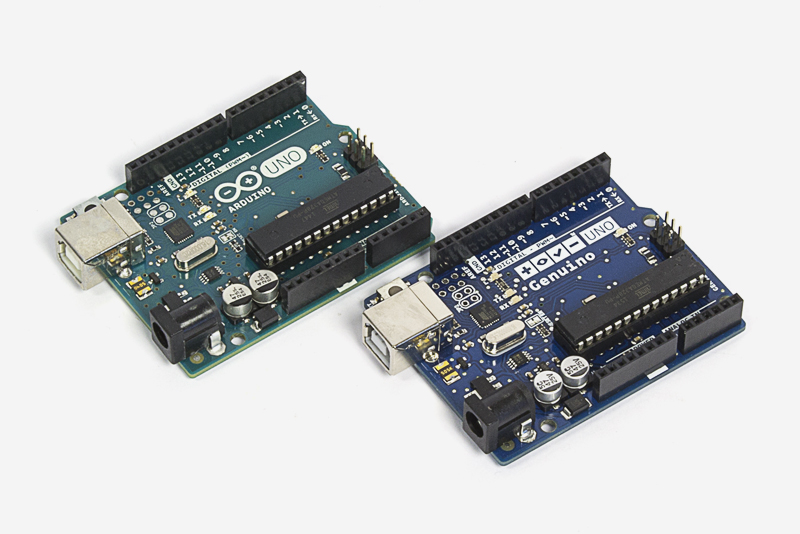
\includegraphics[height=0.4\textwidth]{images/uno.jpg}
    \caption{Arduino Uno \label{Arduino Uno}}
    \source{\url{https://www.arduino.cc/en/Main/ArduinoBoardUno}\cite{ArduinoUno}}
\end{figure}

Największą zaletą Arduino jest charakterystyczne i zawsze takie same rozmieszczenie dostępnych pinów. Z tego powodu wielu producentów w swoich produktach uwzględnia to rozmieszczenie przez co podłączenie zewnętrznych komponentów jest bardzo proste i wygodne.

Najczęściej spotykane wrsje Arduino to:
Intel Galileo zostało wyposażone w:
\begin{enumerate}
  \item Arduino Uno - najbardziej podstawowa wersja
  \item Arduino Leonardo
  \item Arduino Mega - wersja z dużo większą ilością wejść GPIO
  \item Arduino Pro
\end{enumerate}

W standardzie TTL\footnote{ang. Transistor-transistor logic} wartość logiczna 1 równa jest napięciu 5V, a wartość 0 odpowiada napięciu 0V. W Arduino odpowiednikiem tego są wartości \emph{HIGH} oraz \emph{LOW}.
 
\subsection{Intel Galileo}
Zestaw Intel Galileo jest  to mikrokomputer oparty na 32-bitowym procesorze Intel® Quark SoC X1000 i taktowaniu 400MHz. Posiada on standardowy interfejs Arduino składający się z: 14 pinów cyfrowych (w tym 6 pinów mogących pełnić funkcję \emph{PWM}\footnote{ang. Pulse-Width Modulation - technika pozyskiwania wyników analogowych poprzez użycie wyjść cyfrowych}) oraz 6 pinów analogowych. Każdy z tych pinów jest w stanie operować napięciem od 0V do max 5V.

Intel Galileo zostało wyposażone w:
\begin{enumerate}
  \item Wbudowaną kartę sieciową 10/100, 
  \item Port \emph{RS-232} oraz \emph{USB},
  \item Złącze mini PCI Express,
  \item Przetwornik analogowo-cyfrowy,
  \item \emph{SPI} oraz $I^2C$,
  \item RTC\footnote{ang. Real-Time Clock - Zegar czasu rzeczywistego}
  \item UART\footnote{ang. Universal Asynchronous Receiver and Transmitter - układ używany do asynchronicznego przekazywania informacji poprzez port szeregowy},
  \item Slot karty \emph{microSD}.\cite{GalileoBook}
\end{enumerate}

\begin{figure}[!h]
    \centering
    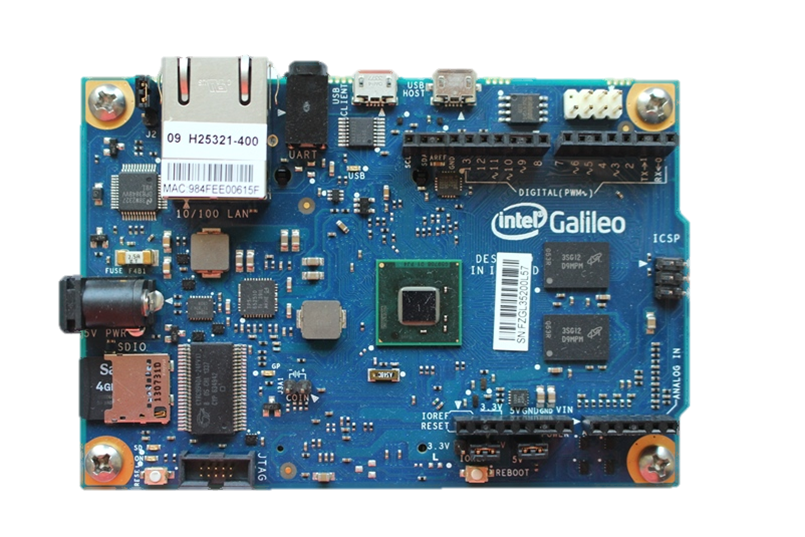
\includegraphics[height=0.4\textwidth]{images/galileo.png}
    \caption{Galileo Gen 1 Board \label{Galileo Gen 1 Board}}
    \source{\url{http://www.intel.com/content/www/us/en/embedded/products/galileo/galileo-g1-datasheet.html}\cite{GalileoBoard}}
\end{figure}

Do komunikacji z Intel Galileo programista ma do dyspozycji port RS-232, USB (działające w trybie host oraz client) oraz wyjście Ehernet. Intel Galileo jest zasilane napięciem 5V 2.0A, które może zostać dostarczone poprzez zasilacz z zestawu lub poprzez podłączenie zasilania do portów PWR\footnote{Port używany jako port zasilania (5V)} oraz GND\footnote{Port używany jako masa - GROUND}. Standardowym środowiskiem programistycznym mikrokomputera jest Intel Arduino Studio. Programista pisząc w języku C i używając dostarczonych przez producenta Arduino funkcji do obsługi portów może się z nimi komunikować. Następnie przesyła skompilowaną wersję oprogramowania poprzez kabel USB do urządzenia. Po przesłaniu program zostaje załadowany do pamięci urządzenia i uruchomiony. 

Standardowo w Intel Galileo znajduje się podstawowa wersja systemu mini Linux. Użytkownik może jednak użyć własnego obrazu systemu uruchamiając go z karty pamięci. Komunikację z systemem operacyjnym można prowadzić w dowolnym języku programowania (np. C, NodeJS, python) łącząc się poprzez dowolny port komunikacyjny na przykład: SSH\footnote{ang. secure shell - protokół komunikacyjny służący do połączenia się ze zdalnym komputerem będącym w sieci} lub port RS-232.

\begin{figure}[!h]
    \centering
    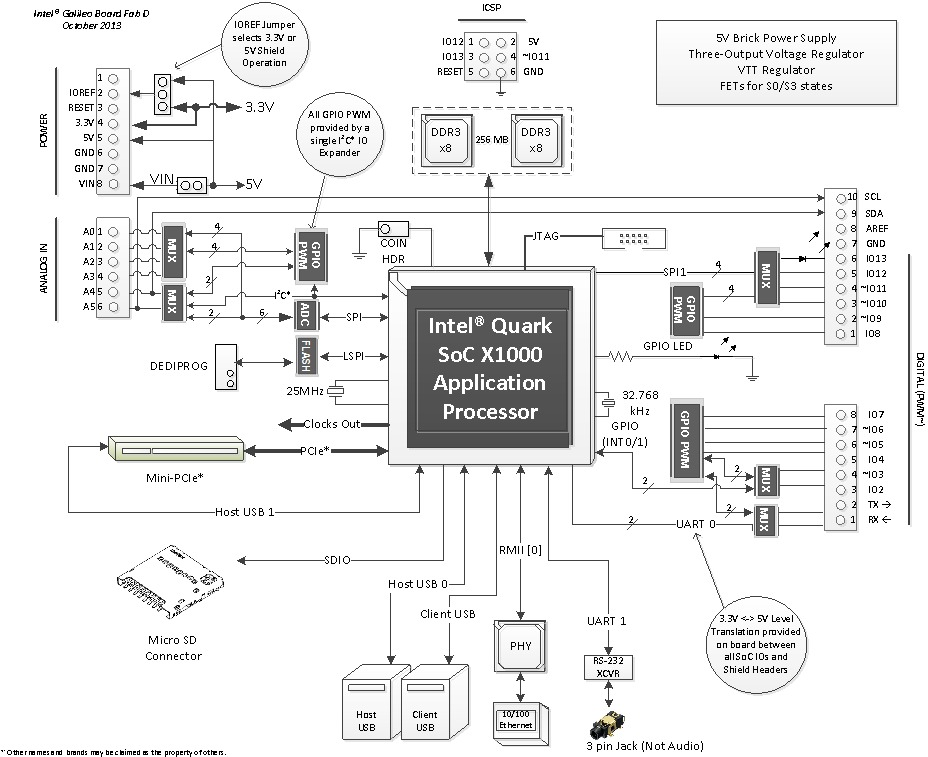
\includegraphics[height=0.6\textwidth]{images/IntelGalileoLogicSchematics.jpg}
    \caption{Schemat logiczny układu Intel Galileo\label{IntelGalileoLogicSchematics}}
    \source{\url{https://www.arduino.cc/en/ArduinoCertified/IntelGalileo}\cite{IntelGalileo}}
\end{figure}

\subsection{FDTI EVE VM800B}
Do komunikacji komputera z użytkownikiem został użyty wyświetlacz \emph{TFT FDTI EVE VM800B} wraz z panelem dotykowym oraz wbudowanym kontrolerem audio. 

Podstawowe cechy urządzenia\cite{FTDI}:
\begin{enumerate}
	\item Pojedynczy układ scalony dla wyświetlacza oraz kontrolera Audio
	\item Ekran 3.5" TFT
	\item Możliwość wyświetlania grafiki xx bitowej
	\item Możliwość komunikacji poprzez użycie interfejsu $I^2C$ lub SPI
	\item Wbudowany system HMI\footnote{ang. Human - Machine Interface} - system bazujący na widgetach umożliwiający stworzenie interfejsu pomiędzy użytkownikiem a systemem w bardzo prosty oraz wygodny sposób.
\end{enumerate}

\begin{figure}[!h]
    \centering
    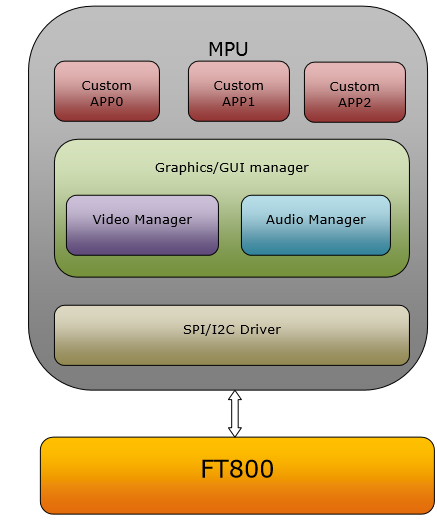
\includegraphics[height=0.3\textheight]{images/FTDIarchitecture.png}
    \caption{Architektura Ekranu FTDI EVE VM800B}
    \source{FT800 Programmers Guide}
\end{figure}

Rozpoczęcie pracy wyświetlacza polega na zainicjalizowaniu go poprzez wpisanie określonych przez specyfikację producenta wartości do określonych obszarów jego pamięci określając w ten sposób np. rozdzielczość lub włączenie/wyłącznie modułu odpowiedzialnego za dźwięk czy dotyk. 

Kolejnym krokiem jest wywołanie zestawu funkcji odpowiedzialnych za rysowanie niezbędnych do działania systemu elementów np. guzików. Wszystkie wyświetlane elementy są na początku zapisywane w kołowym buforze pamięci. Następnie gdy cały ekran zostanie już przygotowany następuje wyświetlenie wszystkiego co zostało zapisane do bufora po czym zostaje on wyczyszczony. Należy pamiętać, że wielkość bufora, którą mamy do dyspozycji wynosi 4 Kb.

Procedura rysowania wygląda następująco:
\begin{enumerate}
	\item Poczekaj aż wszystko co miało zostać wyświetlone, zostanie wyświetlone - opróżnij bufor
	\item Określ co będzie rysowane - np. linia lub kropka i dodaj to do bufora i przesuń się o 4 bajty w buforze
	\item Ustaw wszystkie potrzebne parametry - np. wielkość, kolor lub położenie i dodaj to do bufora, pamiętając aby za każdym razem przesunąć się o 4 bajty w buforze
	\item Wyświetl wszystko do zostało dodane do bufora kołowego 
\end{enumerate}

\begin{figure}[!h]
    \centering
    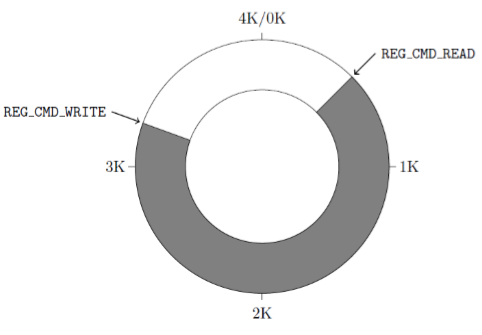
\includegraphics[height=0.25\textheight]{images/buf.png}
    \caption{Bufor kołowy dostępny podczas programowania ekranu VM800}
    \source{FT800 Programmers Guide}
\end{figure}

Komunikacja Galileo z Ekranem odbywa się poprzez protokół komunikacyjny \emph{SPI} (Protokół ten został opisany w części \emph{"Implementacja"}).

\begin{figure}[!h]
    \centering
    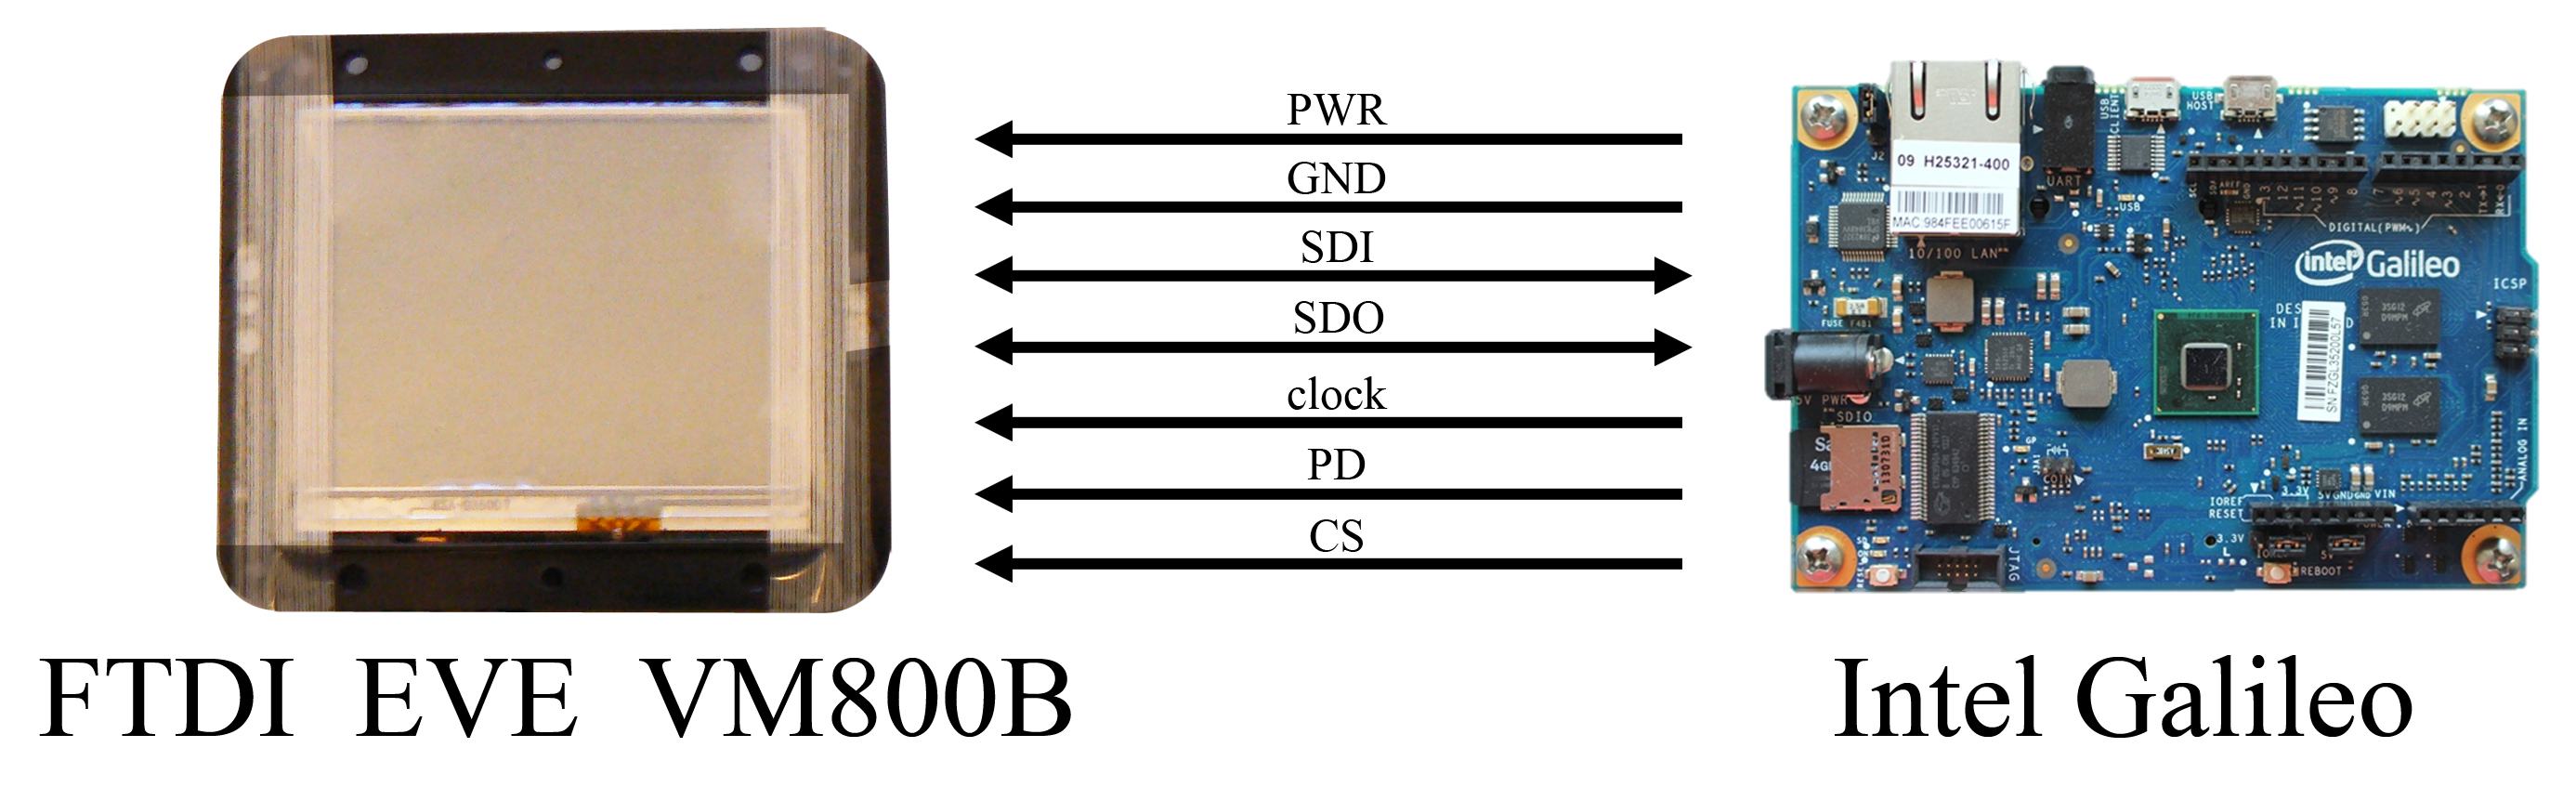
\includegraphics[height=0.24\textheight]{images/ekranGalileo.jpg}
    \caption{Schemat połączenia wyświetlacza FTDI EVE z Intel Galileo za pomocą SPI}
    \source{Opracowanie własne}
\end{figure}

\subsection{Symulator samochodu}
Do celów demonstracyjnych oraz implementacji komputer nie został zamontowany w fizycznym samochodzie. Zamiast tego został zbudowany symulator samochodu mający obrazować pełną pracę pojazdu.

\begin{figure}[!h]
    \centering
    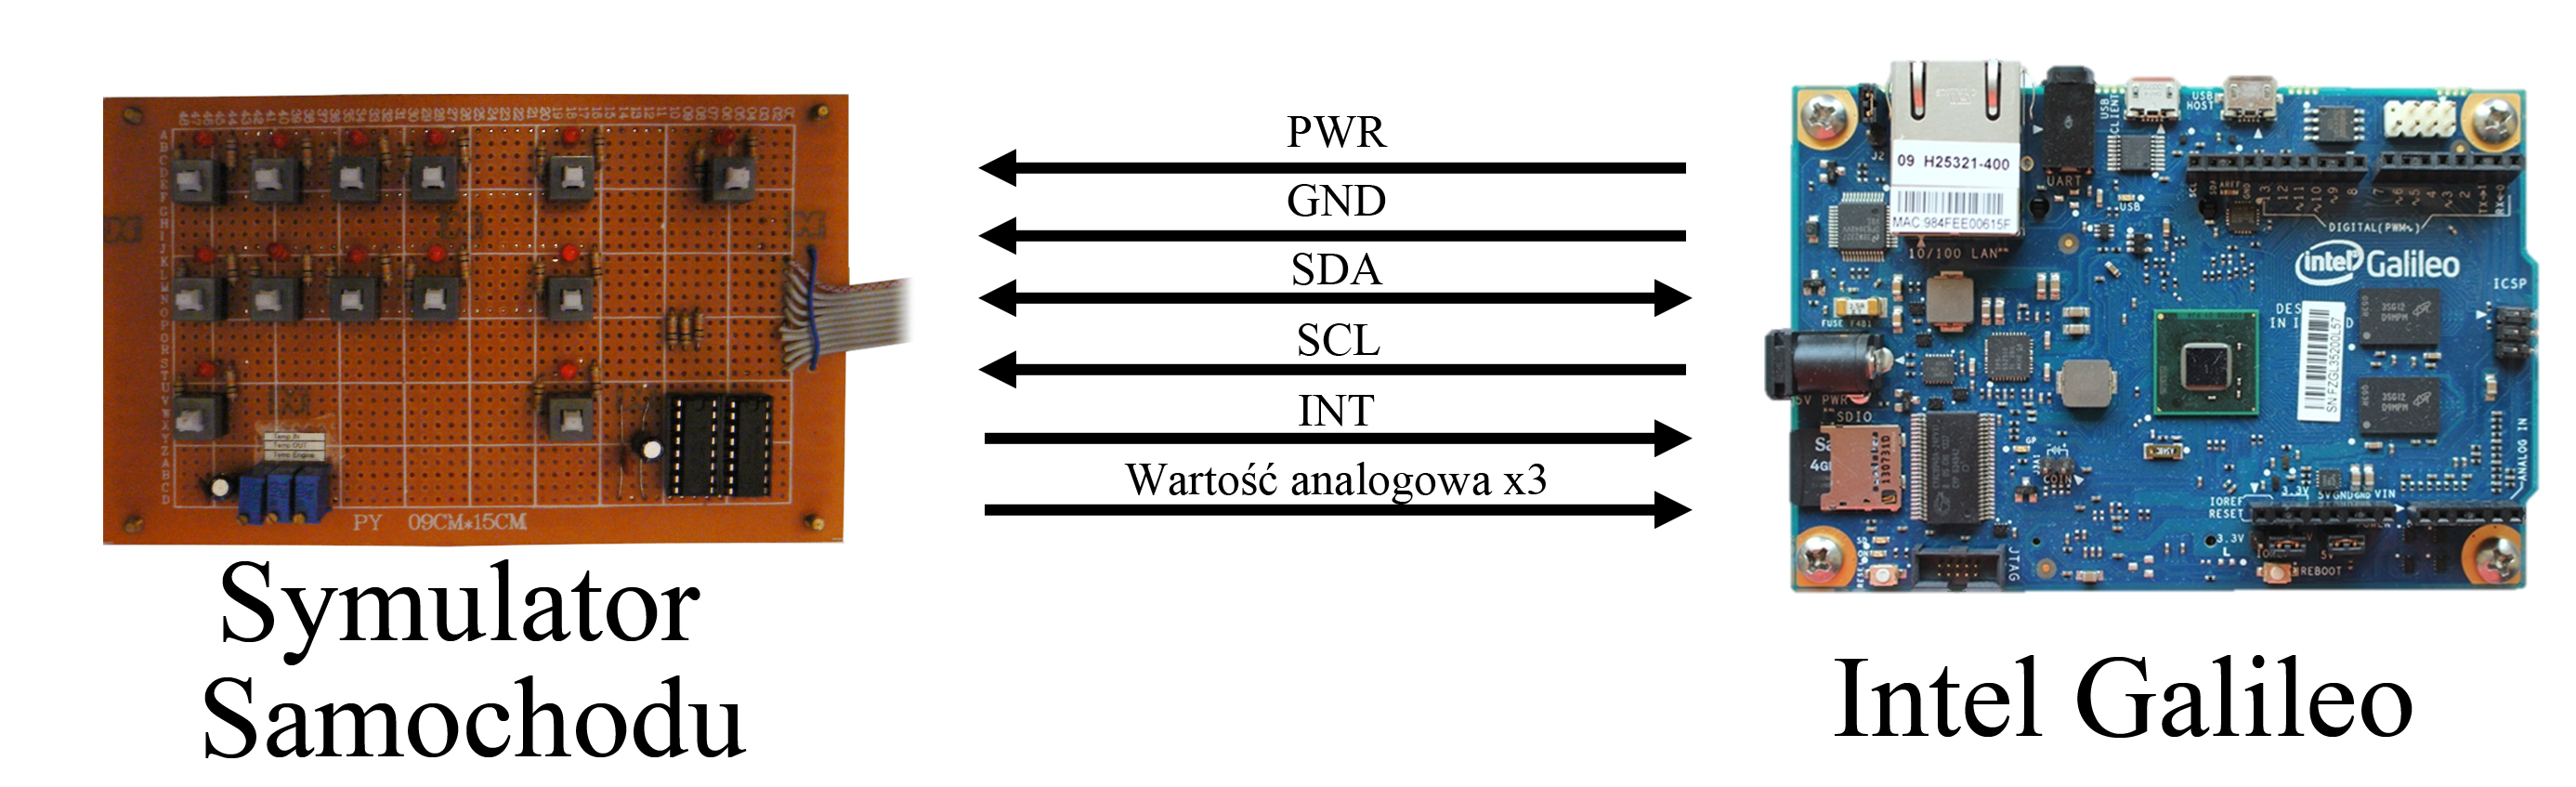
\includegraphics[height=0.24\textheight]{images/symulatorGalileo.jpg}
    \caption{Schemat połączenia symulatora samochodu z Intel Galileo za pomocą $I^2C$}
    \source{Opracowanie własne}
\end{figure}

Symulator składa się z:
\begin{enumerate}
	\item 11 przełączników bistabilnych symulujących stan drzwi samochodu (wraz z stanem bagażnika), pasy pasażerów, przełączenie biegu na wsteczny oraz włączenie świateł - wciśniecie przełącznika dodatkowo obrazowane jest poprzez zaświecenie diody półprzewodnikowej
	\item 2 I/O Expandery PCF 8574N 
	\item 3 potencjometrów symulujących czujniki temperatury w samochodzie
\end{enumerate}

Przełączniki wysyłają sygnały cyfrowe, a potencjometry sygnały analogowe. Ze względu na znaczną ilość sygnałów cyfrowych wychodzących z symulatora komunikacja z Galileo odbywać się będzie poprzez \emph{I/O Expander PCF 8574N} wykorzystujący protokół  $I^2C$ (Protokół ten został opisany w części \emph{"Implementacja"}).
%================KONIEC Architektura=====================

%================Mechanizmy komunikacji systemu mikroprocesorowego z otoczeniem=====================
\chapter{Mechanizmy komunikacji systemu mikroprocesorowego z otoczeniem}
\subsection{Porty}
Porty najczęściej dzieli się na:
\begin{enumerate}
	\item Cyfrowe
	\item Analogowe
\end{enumerate}

Porty cyfrowe charakteryzują się możliwością przyjęcia lub wysłania sygnału binarnego (1 - jest sygnał, 0 - sygnału nie ma). Najczęściej wysłanie sygnału równego 1 jest równoznaczne z wysłaniem napięcia o wartości 5V oraz odpowiednio wysłanie 0 jest równoznaczne z wysłaniem napięcia równego 0V. Z kolei porty analogowe mogą przesyłać sygnały o większej ilości danych lecz do ich obsługi konieczny jest przetwornik analogowo-cyfrowy, który w Intel Galileo jest 10 bitowy - co oznacza możliwość wysłania jednorazowo do 10 bitów danych. Każdy z portów może działać w jednym  z dwóch trybów: wejścia - oczekiwać na przyjęcie danych od urządzenia zewnętrznego lub wyjścia - wysyłać dane do urządzenia zewnętrznego.

\subsection{Odpytywanie w pętli}
Jednym z najprostszych metod pozyskania danych z urządzeń wejścia/wyjścia mikro kontrolera jest odpytywanie urządzeń zewnętrznych w nieskończonej pętli. Jest to najmniej efektywny sposób ponieważ większość czasu zajmuje zasoby sprzętu zapytaniami, które nie zawsze są konieczne. Odczyt stanu urządzeń wejścia/wyjścia może być realizowane mechanizmami systemu operacyjnego (wykorzystując gotowe biblioteki np. Arduino/Wire) lub niskopoziomowo z wykorzystaniem funkcji języka C i/lub Asemblera.

\subsection{Przerwania}
Podobnym mechanizmem do odpytywania w pętli jest mechanizm przerwań. 

Przerwanie na poziomie procesora jest to sygnał elektryczny pochodzący bezpośrednio z urządzeń do mikroprocesora.

Są to bezpośrednie funkcje systemu lub sprzętu ułatwiające komunikację ze światem zewnętrznym. Część z nich jest zarezerwowana przez system lecz część jest wolna do wykorzystania przez programistę.

System Galileo bazując na procesorze Quark ma standardowy dla produktów Intela mechanizm obsługi przerwań obsługiwany za pomocą kontrolera przerwań, którego działanie i konstrukcją jest zbliżona do rozwiązań stosowanych w IBM PC/ATX więc do dyspozycji mamy przerwania:
\begin{enumerate}
	\item Programowe
	\item Sprzętowe
	\begin{enumerate}
		\item Niemaskowalne (NMI\footnote{Non-Maskable Interrupt})
		\item Maskowalne
	\end{enumerate}
	\item Wyjątek
\end{enumerate}

W momencie gdy zostaje zgłoszone przerwanie wątek programu zostaje zatrzymany po czym wykonywany jest skok do odpowiedniej funkcji.

Przerwania programowe wywołuje się za pomocą instrukcji asemblera \emph{INT XX}, gdzie \emph{XX} oznacza numer przerwania zadeklarowanego w tablicy wektorów przerwań\footnote{ang. interrupt vector table - tablica zawierająca adresy podprogramów służących do obsługi wektorów przerwań}, która jest tworzona przy każdorazowym starcie systemu. W IAPX znajduje się 255 wektorów przerwań.

Przerwanie sprzętowe jest to rodzaj przerwań wywoływanych przez urządzenia wejścia/wyjścia lub zgłaszane przez procesor. Efektem zgłoszenia przerwania sprzętowego jest obsłużenie go poprzez wywołanie przerwania programowego. Przerwania te dzielimy na maskowalne oraz niemaskowalne. Główna różnica między nimi polega na możliwości zablokowania przerwań maskowalnych podczas gdy przerwania niemaskowalne muszą zostać obsłużone. Przykładem przerwania niemaskowalnego w systemach IAPX 86 jest \emph{INT2}, który w środowisku Windows znany jest jako popularny \emph{Blue Screen of Death}\footnote{Ekran błędu w systemach Windows pojawiający się po krytycznym błędzie systemu}.

Ostatnim rodzajem przerwań są wyjątki. Wywoływane są podczas napotkania przez procesor błędów oraz niepowodzeń.
%================KONIEC Mechanizmy komunikacji systemu mikroprocesorowego z otoczeniem=====================

%================Programowanie z użyciem rożnych środowisk=====================
\chapter{Programowanie Intel Galileo z użyciem rożnych środowisk}
\section{Programowanie w środowisku Intel Arduino studio}
Programy pisane w środowisku Arduino różnią się nieznacznie od klasycznych programów pisanych w języku C. 

\begin{figure}[!h]
    \centering
    	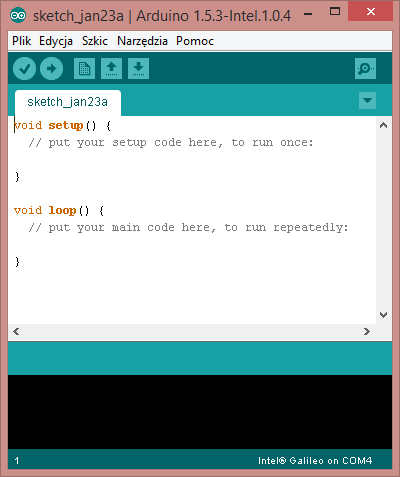
\includegraphics[height=0.3\textheight]{images/AS.png}
    \caption{Arduino Studio}
    \source{Opracowanie własne}
\end{figure}

Pierwszą różnicą jest jednorazowe wywołanie funkcji \emph{setup()} zaraz po przesłaniu i uruchomieniu programu, która służy do inicjalizacji wszystkich niezbędnych portów. W tej funkcji należy określić początkowe tryby pracy portów. Następnie wywołana zostaje funkcja \emph{loop()}, która jest równoznaczna z funkcją \emph{main()} w języku C, z tą różnicą, że jest wykonywana od momentu startu (zaraz po jednorazowym wykonaniu funkcji \emph{setup()}) aż do wyłączenia systemu. Taką sytuację można utożsamiać z wywołaniem jakiejkolwiek funkcji w bloku \emph{while(1)}.

\begin{lstlisting}[label=bot-dirs-alg,caption=Odpytywanie funkcji w nieskończonej pętli w środowisku Arduino]
void loop() {
	funcName();
	delay(1000);
}
\end{lstlisting}

W środowisku \emph{Arduino} aby obsłużyć port cyfrowy wystarczy ustalić tryb w jakim ma on działać (wejście/wyjście), a następnie wysłać/odczytać dane.

Wpisanie wartości \emph{LOW} jest równoznaczna z wysyłaniem napięcia 0V na określonym pinie, a wpisanie wartości \emph{HIGH} jest równoznaczna z wysyłaniem napięcia 5V na określonym pinie.

Arduino dostarcza funkcje do obsługi portów. Podstawowe z nich to:

\begin{enumerate}
	\item \emph{pinMode(PIN, MODE);} - funkcja ustawiająca pin o podanym numerze (PIN) na podany tryb pracy - wejście/wyjście (MODE)
	\item \emph{digitalWrite(PIN, VAL);} - funkcja wpisująca wartość (VAL) - HIGH/LOW - do podanego portu cyfrowego (PIN)
	\item \emph{digitalRead(PIN);} - funkcja czytająca wartość z podanego portu cyfrowego (PIN)
	\item \emph{analogWrite(PIN, VAL);} - funkcja wpisująca wartość (VAL) do podanego portu analogowego (PIN)
	\item \emph{analogRead(PIN);}  - funkcja czytająca wartość z podanego portu analogowego (PIN)
\end{enumerate}

\begin{lstlisting}[label=bot-dirs-alg,caption=Obsługa portu cyfrowego w środowisku Arduino]
int val = 0;
int digitalPin = 1;	
pinMode(digitalgPin, INPUT);
val = digitalRead(digitalPin);
pinMode(digitalPin, OUTPUT);
digitalWrite(digitalPin, HIGH);
\end{lstlisting}

\begin{lstlisting}[label=bot-dirs-alg,caption=Obsługa portu analogowego w środowisku Arduino]
int val = 2;
int analogPin = A1;	
pinMode(analogPin, INPUT);
val = analogRead(analogPin);
pinMode(analogPin, OUTPUT);
analogWrite(ledPin, val);
\end{lstlisting}

Arduino oczywiście obsługuje przerwania. W środowisku Arduino aby zainicjalizować przerwania wystarczy wywołać funkcję \emph{attachInterrupt}:

\begin{lstlisting}[label=bot-dirs-alg,caption=Obsługa przerwań sprzętowych w środowisku Arduino]
void setup(){
	attachInterrupt(pinInt, funcName, mode);
}
\end{lstlisting}
gdzie \emph{pinInt} jest to pin na którym Arduino będzie nasłuchiwało na przerwanie, \emph{funcName} jest to nazwa funkcji, która zostanie wykonana gdy przerwanie zostanie zgłoszone, \emph{mode} jest to określenie kiedy sygnał może być uznany za przerwanie. Należy pamiętać, że funkcja wywoływana przez przerwanie nie może przyjmować żadnych parametrów oraz zwracać żadnego wyniku. \emph{Mode} może przyjmować wartości:
 
\begin{enumerate}
	\item LOW - przerwanie zostanie zgłoszone gdy wartość na określonym pinie jest równa LOW
	\item CHANGE - przerwanie zostanie zgłoszone gdy wartość na określonym pinie zostanie zmieniona
	\item RISING - przerwanie zostanie zgłoszone gdy wartość na określonym pinie zostanie zmieniona z LOW na HIGH
	\item FALLING - przerwanie zostanie zgłoszone gdy wartość na określonym pinie zostanie zmieniona z HIGH na LOW
\end{enumerate}

Mechanizmem, który bazuje na przerwaniach jest mechanizm Timera. Polega on na wywołaniu funkcji co określony czas (zgłaszane jako przerwanie), którego zarządzaniem zajmuje się urządzenie (lub system operacyjny). Rozwiązanie to jest bardzo podobne do odpytywania w pętli, a następnie wywołania funkcji \emph{delay()} z tą różnicą, że użycie timera jest dokładniejsze ponieważ wykorzystuje zegar czasu rzeczywistego znajdującego się w CPU\footnote{ang. Central Processing Unit - jednostka arytmetyczno-logiczna wykorzystywana do wykonywania obliczeń niezbędnych do działania programu}.
\begin{lstlisting}[label=bot-dirs-alg,caption=Przykładowe użycie timer w środowisku Arduino]
#include <TimerOne.h>
void setup(){
	Timer1.initialize(500000);
	Timer1.attachInterrupt(funcName, 500000);
}
\end{lstlisting}

\section{Komunikacja z urządzeniami poprzez mechanizmy systemu operacyjnego Linux YOCTO}
Z punktu widzenia systemu operacyjnego Linux YOCTO urządzenia są traktowane tak jak pliki. W systemie YOCTO Linux dostępne są pliki w katalogu /sys/class/gpio/ odpowiadające poszczególnym portom w Galileo. Przy komunikacji należy jednak pamiętać, że nazwy urządzeń nie są intuicyjne tzn. port IO4 nie jest plikiem \emph{/sys/class/gpio/gpio4} (Patrz Dodatek C). Komunikację z portami można obrazować jako wpisanie lub odczytanie danych z pliku. Na początku należy ustalić w jakim trybie ma działać port. W tym celu do pliku \emph{/sys/class/gpio/PORT/direction} należy wpisać wartość \emph{out} dla ustawienia jako wyjście lub \emph{in} dla ustawienia jako wejście. Następnie można odczytać lub wpisać dane do wcześniej skonfigurowanego portu. W tym celu do pliku \emph{/sys/class/gpio/PORT/value} należy wpisać wartość \emph{1} dla ustawienia stanu wysokiego - odpowiednik \emph{HIGH} z Arduino lub \emph{0} dla ustawienia stanu niskiego - odpowiednik \emph{LOW} z Arduino, gdzie \emph{PORT} jest to numer odpowiedniego portu według numeracji Galileo. Warto zauważyć, że przesyłane wartości tym mechanizmem nie są wartościami 8 tylko 1 bitowymi.

Dla języka C wygląda to następująco:
\begin{lstlisting}[label=bot-dirs-alg,caption=Obsługa portu cyfrowego w środowisku Linux (język C)]
FILE *fp;
int value;

// Ustawienie portu cyfrowego nr 13 jako port wyjscia
fp = fopen("/sys/class/gpio/gpio39/direction", "w");
fprintf(fp, "out");
fclose(fp);

// Wpisanie wartosci do portu cyfrowego
fp = fopen("/sys/class/gpio/gpio39/value", "w");
fprintf(fp, "1");
fclose(fp);

// Odczytanie wartosci z portu cyfrowego
fp = fopen("/sys/class/gpio/gpio39/value", "r");
fscanf(fp, "%i", &value);
fclose(fp);
\end{lstlisting}

oraz podobnie dla języków skryptowych np. Bash:

\begin{lstlisting}[label=bot-dirs-alg,caption=Obsługa portu cyfrowego w środowisku Linux (bash)]
# Ustawienie portu cyfrowego nr 13 jako port wyjścia
root@henio:~# echo -n "out" > /sys/class/gpio/gpio39/direction

# Wpisanie wartosci do portu cyfrowego
root@henio:~#  echo -n "0" > /sys/class/gpio/gpio39/value
root@henio:~#  echo -n "1" > /sys/class/gpio/gpio39/value

# Odczytanie wartosci z portu cyfrowego
root@henio:~# echo -n "in" > /sys/class/gpio/gpio28/direction
root@henio:~# cat /sys/class/gpio/gpio28/value
\end{lstlisting}

Należy pamiętać aby najpierw ustalić tryb w jakim ma działać port. W przypadku ustawienia portu w tryb wyjścia - \emph{OUT} - gdy nie zostanie to zrobione przed próbą wpisania wartości to otrzymamy błąd: \emph{write error: Operation not permitted}.

%================KONIEC Programowanie z użyciem rożnych środowisk=====================

%================IMPLEMENTACJA=====================
\chapter{Implementacja}
\section{Protokół komunikacyjny $I^2C$}
Protokół komunikacyjny \emph{$I^2C$}\footnote{ang. Inter-Integrated Circuit} jest szeregowym interfejsem stworzonym przez firmę \emph{Philips} służącym do przesyłania danych między urządzeniami elektrycznymi. W projekcie protokół ten został użyty do komunikacji z I/O Expander PCF 8574N.

\begin{figure}[!h]
    \centering
    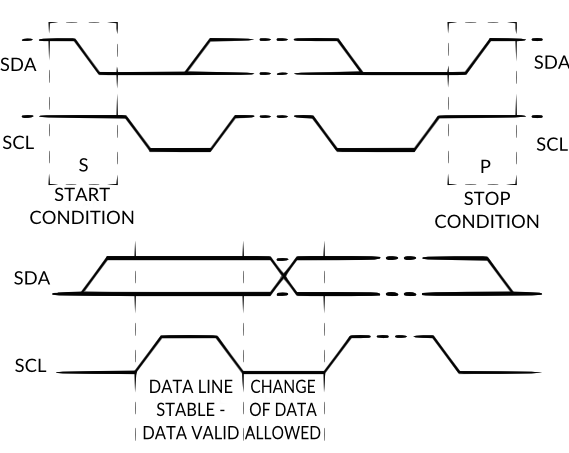
\includegraphics[height=0.3\textheight]{images/i2c.png}
    \caption{Przebieg czasowy protokołu $I^2C$}
    \source{\url{http://www.byteparadigm.com/applications/introduction-to-i2c-and-spi-protocols/}\cite{byteparadigm}}
\end{figure}

Podstawową cechą \emph{$I^2C$} jest wykorzystywanie dwóch linii służących do komunikacji: dwukierunkowa linia danych \emph{SDA\footnote{ang. Serial Data Line}} oraz jednokierunkowa linia zegarowa \emph{SCL\footnote{ang. Serial Clock Time}}. Protokół $I^2C$ bazuje na przesyłaniu ramek (pakietów) składających się z sekwencji: START -> adres -> dane -> STOP.

Do wygenerowania impulsu START należy ustawić linię \emph{SDA} oraz \emph{SCL} w stan \emph{HIGH} (5V) po czym w trakcie gdy linia \emph{SCL} jest w stanie \emph{HIGH} należy zmienić stan linii \emph{SDA} na stan \emph{LOW}. Analogicznie do wygenerowania impulsu STOP należy w trakcie gdy linia \emph{SCL} jest w stanie \emph{HIGH} zmienić stan linii \emph{SDA} ze stanu \emph{LOW} na stan \emph{HIGH}. Dane wysyłane/odbierane są bit po bicie - na początku należy ustawić linię \emph{SCL} w stan wysoki (HIGH), odczytać wartość na linii \emph{SDA}, a następnie zmienić stan linii \emph{SCL} na niski (LOW).

Adresowanie urządzenia odbywa się poprzez wysłanie pojedynczych bitów adresu (pamiętając o kolejności MSB->LCB\footnote{Wysyłanie odbywa się w kolejności od najbardziej znaczących (najstarszych) bitów}) oraz wygenerowanie impulsu zegara. Gdy chcemy zaadresować urządzenie, którego adresem jest np. 4 należy wykonać:
\begin{lstlisting}[label=bot-dirs-alg,caption=Własna wersja adresowania urządzenia $I^2C$ na przykładzie PCF8574N]
int adres = 4;
for(m = 0x80; m; m >>= 1){
    if(adres & m)         
      digitalWrite(sda, HIGH);
    else
      digitalWrite(sda, LOW);
        
   digitalWrite(scl, HIGH);
   digitalWrite(scl, LOW); 
}
\end{lstlisting}

Kolejnym krokiem jest ustalenie czy będziemy chcieli z urządzenia przeczytać dane czy je wysłać. W tym celu należy wysłać 1 lub 0  jako kolejny bit. Po otrzymaniu potwierdzenia na linii \emph{SDA} można zacząć komunikację z urządzeniem. Na zakończenia transmisji należy wysłać sygnał \emph{STOP}.

\begin{figure}[!h]
    \centering
    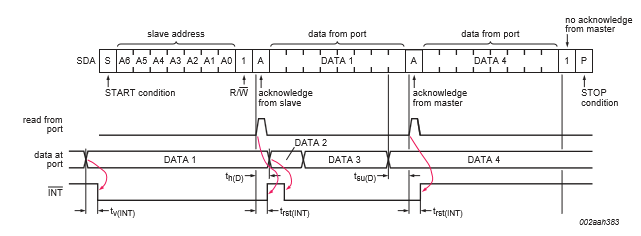
\includegraphics[height=0.25\textheight]{images/read_i2c.png}
    \caption{Schemat odbierania/wysyłania danych poprzez $I^2C$ na przykładzie PCF8574N\label{$I^2C$}}
    \source{Karta katalogowa I/O Expander PCF8574N}
\end{figure}

Dane wysyłane są od najstarszego do najmłodszego bitu. Każda paczka potwierdzona jest przez odbiornik (bit ACK\footnote{ang. Acknowledge}). Należy również pamiętać, aby każdą komunikację z urządzeniem rozpocząć i zakończyć ustawiając linie \emph{SDA} oraz \emph{SCL} w stan nieaktywny (HIGH) - zgodnie z prawidłowym wygenerowaniem impulsu STOP.

Podstawowymi zaletami protokołu są:
\begin{enumerate}
	\item Połączenia składają się tylko z dwóch linii co znacznie ogranicza liczbę kabli wychodzących z urządzenia
	\item Częstotliwość pracy wynosi 400kHz
	\item Dane przesyłane są w kolejności MSB->LSB
	\item Każde urządzenie ma swój adres	
	\item Transmisja jest odporna na zakłócenia zewnętrzne
	\item Bez większych problemów można dodawać oraz odejmować układy korzystające z magistrali
\end{enumerate}

Nazwa $I^2C$ jest nazwą zastrzeżoną przez firmę \emph{Philips} dlatego też w literaturze bardzo często spotyka się określenie \emph{TWI}\footnote{ang. Two Wire Interface}. Jest ono stosowane w mikro kontrolerach firmy \emph{Atmel}. 

Galileo posiada dostarczoną od Arduino bibliotekę do obsługi $I^2C$ jednak podczas próby użycia jej w projekcie wystąpiły problemy z kompatybilnością z używanym sprzętem w związku z tym na potrzeby projektu napisana została własna wersja biblioteki obsługującej komunikację poprzez protokół $I^2C$.

\subsection{I/O Expander PCF8574N}
W symulatorze ze względu na dużą ilość wychodzących sygnałów zastosowano I/O Expander wykorzystujący komunikację poprzez $I^2C$. Do obsługi tego został zamontowane dwa I/O Expandery PCF 8574N zbierające wszystkie sygnały cyfrowe wychodzące z symulatora do Galileo. Dzięki temu zamiast używać dwunastu linii cyfrowych, wykorzystywane są jedynie dwie niezbędne do komunikacji poprzez $I^2C$ (\emph{SDA}, \emph{SCL}) co znacznie ułatwiło dalsze korzystanie z Galileo ze względu na pozostałe wolne porty cyfrowe, które mogą być potrzebne w dalszej części pracy do komunikacji z wyświetlaczem i innymi elementami symulatora. Zaletą tego rozwiązania jest możliwość późniejszego podłączenia większej ilości czujników bez jakiejkolwiek ingerencji w okablowanie Galileo.

\section{Protokół komunikacyjny SPI}
Protokół SPI\footnote{ang. Serial Peripherial Interface} składa się z czterech podstawowych linii - dwóch służących do przesyłania danych w przeciwnych kierunkach, jednej z sygnałem taktującym, synchronizującym transfer danych oraz linii \emph{Chip Select}. \emph{Chip Select} jest odpowiednikiem adresu urządzenia z protokołu $I^2C$. Każde urządzenie podłączone pod system musi mieć osobną linię \emph{Chip Select}. Gdy linia zostanie aktywowana (ustawiona w stan HIGH) można rozpocząć komunikację z wybranym urządzeniem.

Linia MISO\footnote{ang. Master In Slave Out} jest linią wejścia danych dla urządzenia nadrzędnego (master), a wyjściem dla urządzenia podrzędnego (slave), linia MOSI\footnote{ang. Master Out Slave In} jest wyjściem dla urządzenia master, a wejściem dla slave. Linia SCK\footnote{ang. Serial Clock} jest wejściem taktującym zegar. Sygnał taktujący jest zawsze generowany przez układ master. Transmisja danych na obydwu liniach jest zawsze dwukierunkowa i odbywa się jednocześnie - nadanie danych na linii MISO wiąże się z nadaniem danych na linii MOSI. Nie zawsze jednak nadane dane niosą ze sobą informację - najczęściej nadawane informacje płyną w jedną stronę podczas, gdy w tym samym czasie wysyłane zostają puste dane.\cite{Dorra}

\begin{figure}[!h]
    \centering
    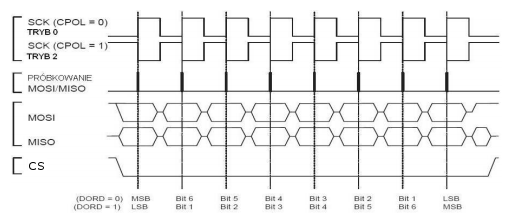
\includegraphics[height=0.25\textheight]{images/spi.png}
    \caption{Przebiegi czasowe interfejsu SPI}
    \source{\url{http://castor.am.gdynia.pl/~dorra}\cite{Dorra}}
\end{figure}

Gdy chcemy wysłać dane 8 bitowe poprzez protokół SPI należy: aktywować odpowiednią linię \emph{Chip Select}, a następnie wysłać dane. Gdy mamy do dyspozycji porty cyfrowe należy to zrobić bit po bicie.
\begin{lstlisting}[label=bot-dirs-alg,caption=Wysłanie danych 8 bitowych za pomocą protokołu SPI]
void sendData(int data, int CS, int clock, int SDO){
  digitalWrite(CS, LOW);
  int i;
  for(i = 0x80; i; i >>= 1){
    digitalWrite(SDO, data & i);
    digitalWrite(clock, HIGH);
    digitalWrite(clock, LOW);
  }
  digitalWrite(CS, HIGH);
}
\end{lstlisting}

\subsection{Komunikacja z ekranem FTDI EVE VM800b poprzez protokół SPI}
Podobnie jak w przypadku protokołu $I^2C$ została napisana własna wersja biblioteki do obsługi protokołu SPI. Do komunikacji niezbędne było napisanie funkcji:
\begin{enumerate}
	\item \emph{void sendData(int data)} - funkcja wysyłająca wartość 8 bitową
	\item \emph{void ft800memWriteX(unsigned long ftAddress, unsigned char ftDataX)} - funkcja wpisująca podaną wartość X - bitową na podany adres, gdzie X może być wartością 8, 16 lub 32 bitową
	\item \emph{unsigned char ft800memReadX(unsigned long ftAddress)} - funkcja odczytująca wartość X - bitową z podanego adresu, gdzie X może być wartością 8, 16 lub 32 bitową
	\item \emph{unsigned int incCMDOffset(unsigned int currentOffset, unsigned char commandSize)} - funkcja zwiększająca offset w buforze pamięci ekranu
	\item \emph{void ft800cmdWrite(unsigned char ftCommand)} - funkcja wysyłająca podaną komendę do ekranu - np. Start urządzenia ($FT800_ACTIVE$)
\end{enumerate}

Wyświetlacz ma możliwość korzystania z systemu \emph{HMI} więc do obsługi zostało napisane proste API, które dostarcza następujące funkcjonalności:
 \begin{enumerate}
	\item inicjalizacja ekranu
	\item rysowanie kółka o podanym rozmiarze, kolorze i w podanym miejscu
	\item rysowanie linii o podanych końcach, szerokości oraz kolorze
	\item wypisanie tekstu
	\item wypisanie cyfr
	\item narysowanie guzika w podanym miejscu i podanym rozmiarze
\end{enumerate}

Przykładowe wyświetlenie linii o pozycji, kolorze oraz szerokościs podanej w parametrach:
\begin{lstlisting}[label=bot-dirs-alg,caption=Narysowanie linii na ekranie]
void linia(unsigned long color, unsigned long x1, unsigned long y1, 
unsigned long x2, unsigned long y2, unsigned long width){
 ft800memWrite32(RAM_CMD+cmdOffset, (DL_BEGIN|LINES));
 cmdOffset=incCMDOffset(cmdOffset, 4);
 
 ft800memWrite32(RAM_CMD+cmdOffset, (DL_COLOR_RGB|color));
 cmdOffset=incCMDOffset(cmdOffset,4);

 ft800memWrite32(RAM_CMD+cmdOffset, (DL_LINE_WIDTH|width));
 cmdOffset=incCMDOffset(cmdOffset,4);

 ft800memWrite32(RAM_CMD+cmdOffset, (DL_VERTEX2F|(x1<<15)|y1));
 cmdOffset=incCMDOffset(cmdOffset,4);
  
 ft800memWrite32(RAM_CMD+cmdOffset, (DL_VERTEX2F|(x2<<15)|y2));
 cmdOffset=incCMDOffset(cmdOffset,4);	
}
\end{lstlisting}

Podobnie gdy chcemy wyświetlić na ekranie kropkę:
\begin{lstlisting}[label=bot-dirs-alg,caption=Narysowanie kropki na ekranie]
void kropka(unsigned long color, unsigned int size, unsigned long x, 
unsigned long y){ 
 ft800memWrite32(RAM_CMD+cmdOffset, (DL_POINT_SIZE|size));
 cmdOffset=incCMDOffset(cmdOffset,4);

 ft800memWrite32(RAM_CMD+cmdOffset, (DL_BEGIN|FTPOINTS));
 cmdOffset=incCMDOffset(cmdOffset, 4);

 ft800memWrite32(RAM_CMD+cmdOffset, (DL_COLOR_RGB|color));
 cmdOffset=incCMDOffset(cmdOffset,4);
 
 ft800memWrite32(RAM_CMD+cmdOffset, (DL_VERTEX2F|(x<<15)|y));
 cmdOffset=incCMDOffset(cmdOffset,4);
}
\end{lstlisting}

%================KONIEC IMPLEMENTACJA=====================

%================Działanie komputera pokładowego=====================
\chapter{Działanie komputera pokładowego}
\section{Założenia funkcjonalne projektu}
Najważniejszym założeniem funkcjonalnym projektowanego systemu była komunikacja z zestawem czujników, które mogą być zamontowane w samochodzie. W projekcie zostały użyte czujniki otwarcia/zamknięcia drzwi, zapięcia pasów, włączenia/wyłączenia świateł oraz czujniki temperatury. Dodatkowym elementem była komunikacja z zewnętrznym wyświetlaczem TFT służącym do komunikacji pomiędzy użytkownikiem a komputerem. Samochód obrazowany został za pomocą zbudowanego symulatora, którego schemat elektryczny został przedstawiony na rysunku 6.2.

\begin{figure}[!h]
    \centering
    	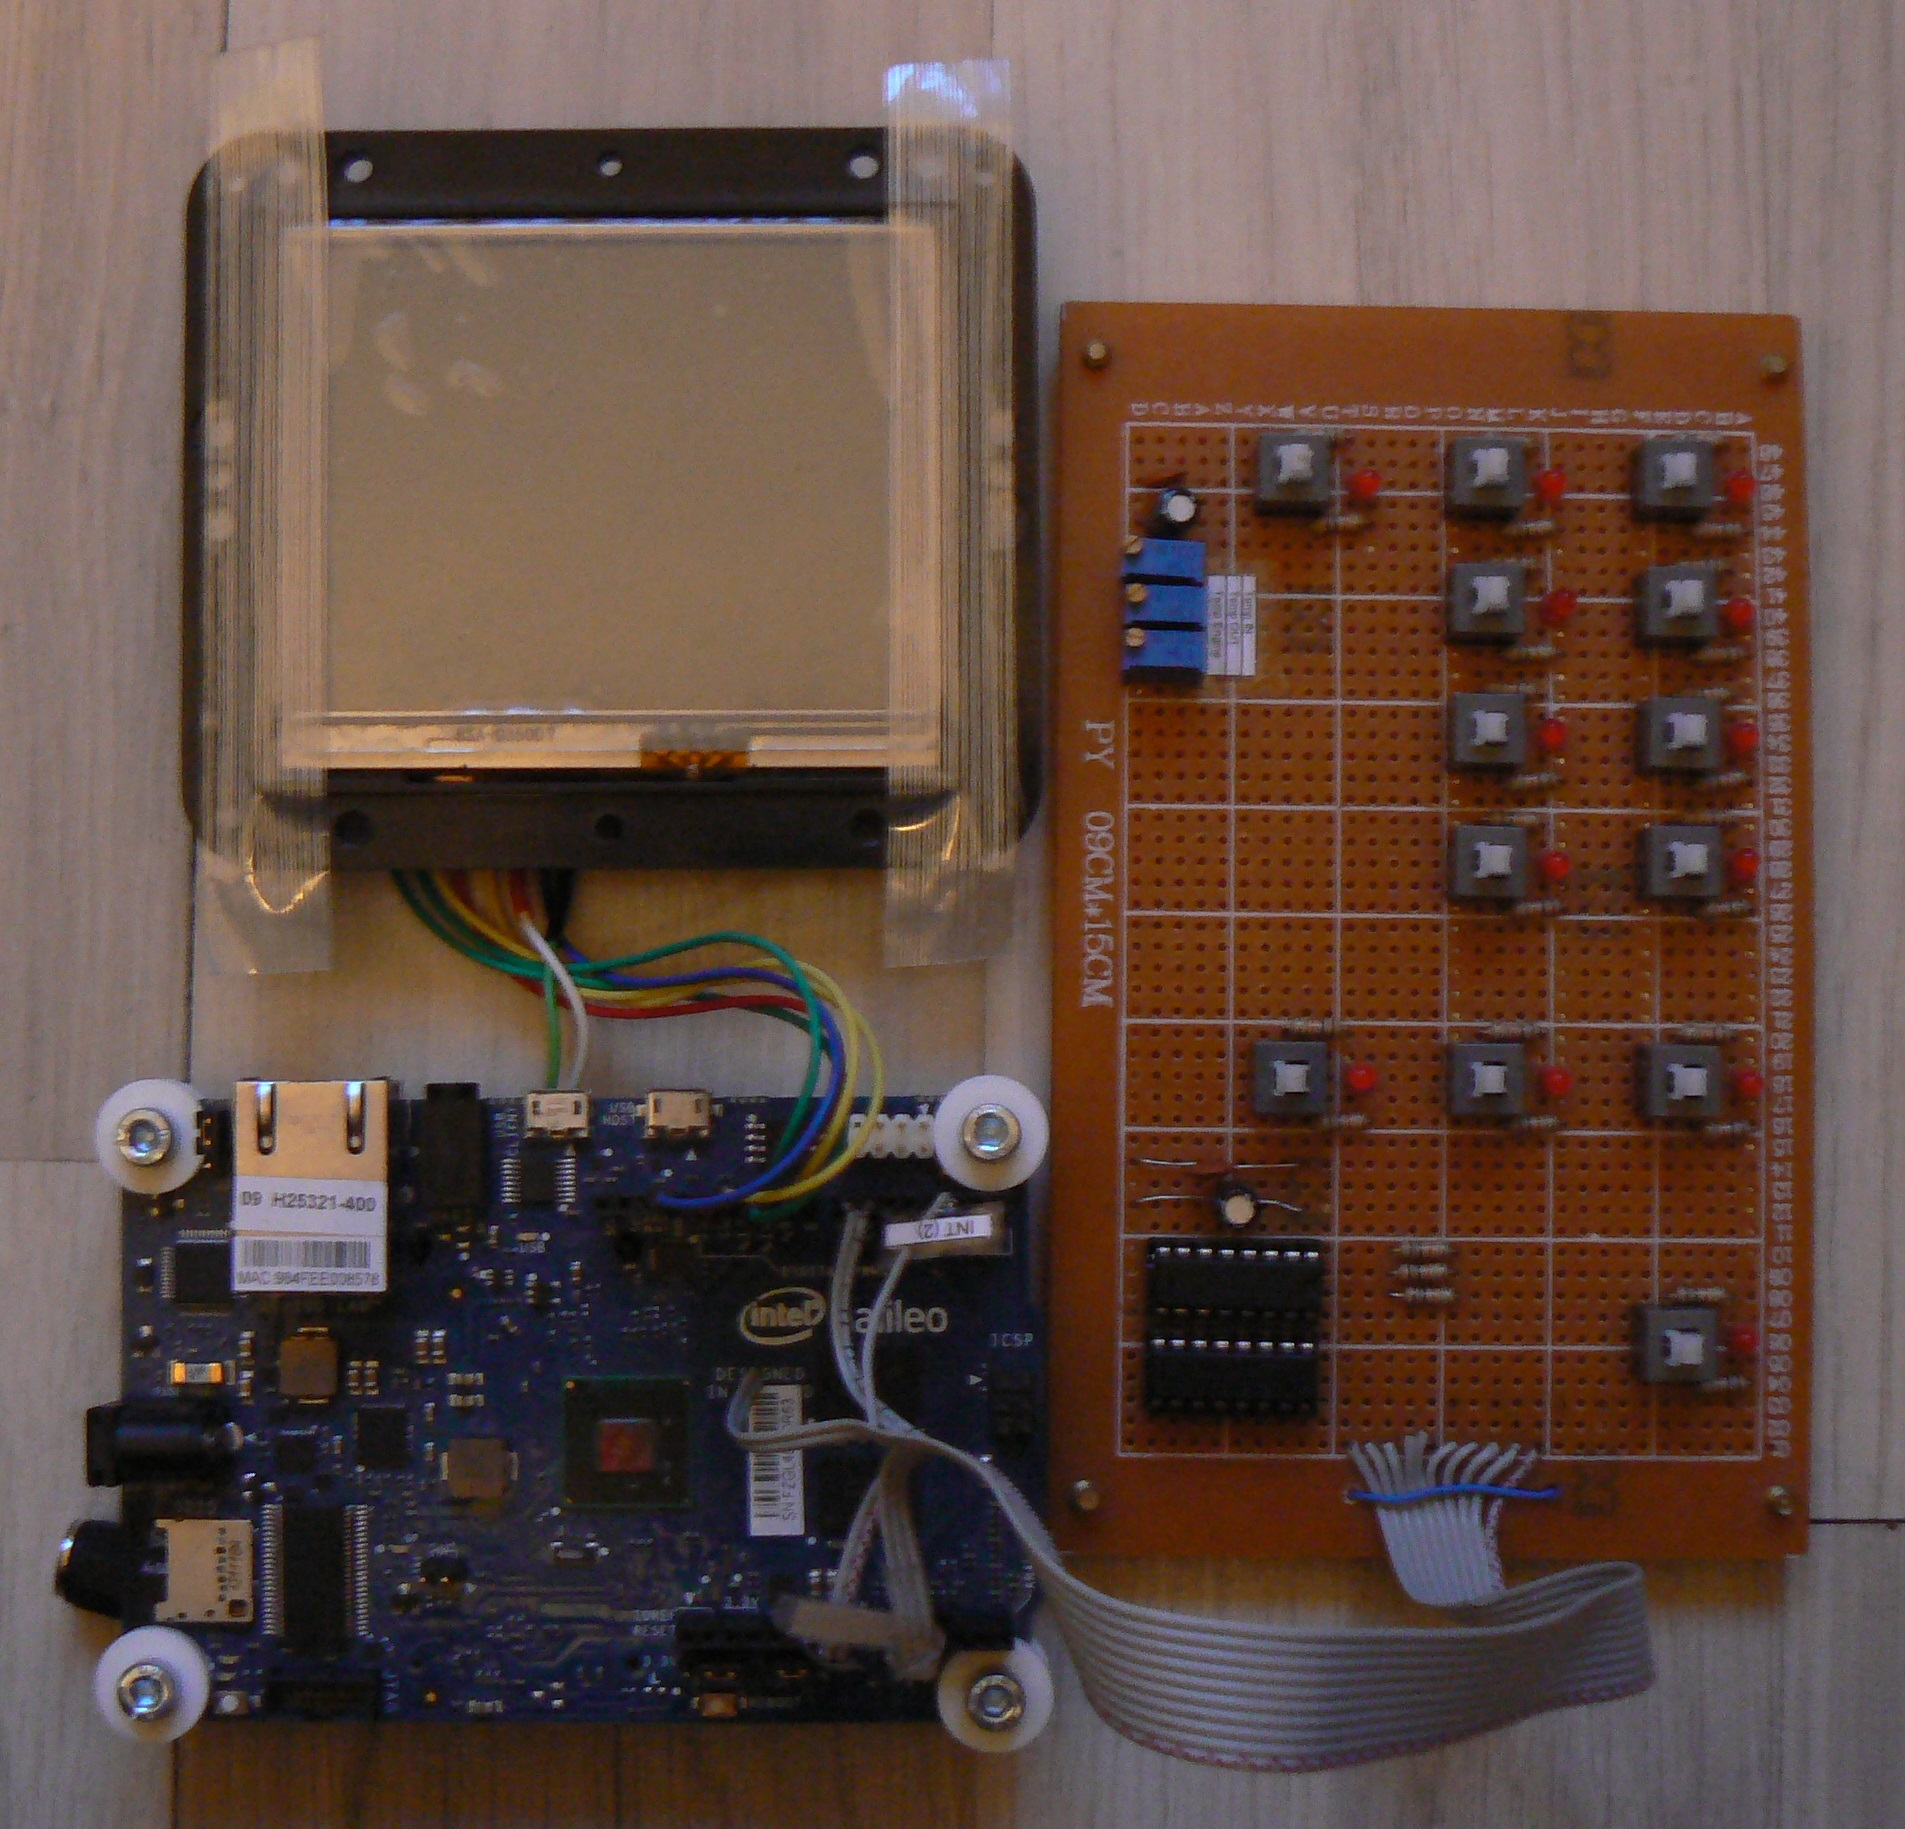
\includegraphics[height=0.35\textheight]{images/zestaw.jpg}
    \caption{Zdjęcie gotowego zestawu}
    \source{Opracowanie własne}
\end{figure}

\begin{figure}[!hp]
    \centering
    	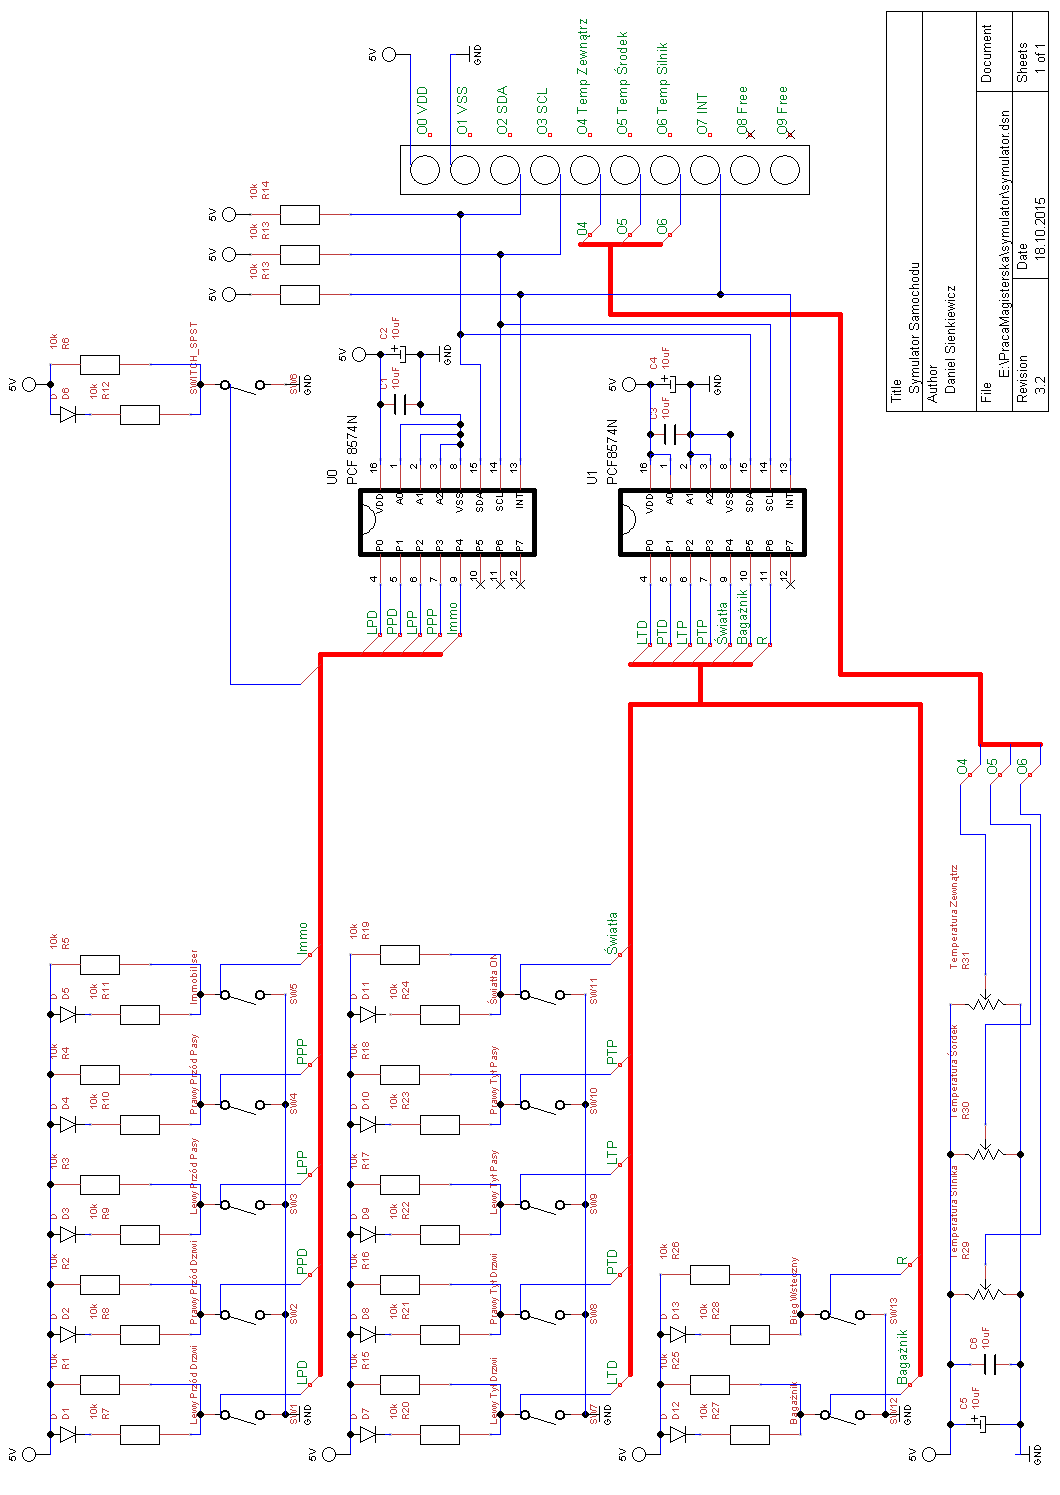
\includegraphics[height=0.9\textheight]{images/symulator.png}
    \caption{Schemat elektryczny symulatora samochodu}
    \source{Opracowanie własne}
\end{figure}

\section{Opis budowy i działania}
Proponowany komputer pokładowy jest całkowicie osobnym systemem niezależnym od sprzętu aktualnie posiadanego w samochodzie. Użytkownik montuje zestaw czujników oraz łączy je z komputerem i ekranem. 

Po wejściu do samochodu oraz włączeniu zapłonu powoduje automatyczny start systemu. 

Na ekranie pojawia się powitanie oraz ekran startowy, na którym można zobaczyć symulację aktualnej pozycji \emph{GPS}, temperaturę panującą w środku samochodu, na zewnątrz oraz w silniku. 

Stan drzwi i pasów z wizualizowany został poprzez miniaturkę samochodu z aktywnie otwierającymi się drzwiami, zapalającymi światłami oraz ikonką obrazującą stan zapiętych pasów.

\begin{figure}[!h]
    \centering
    	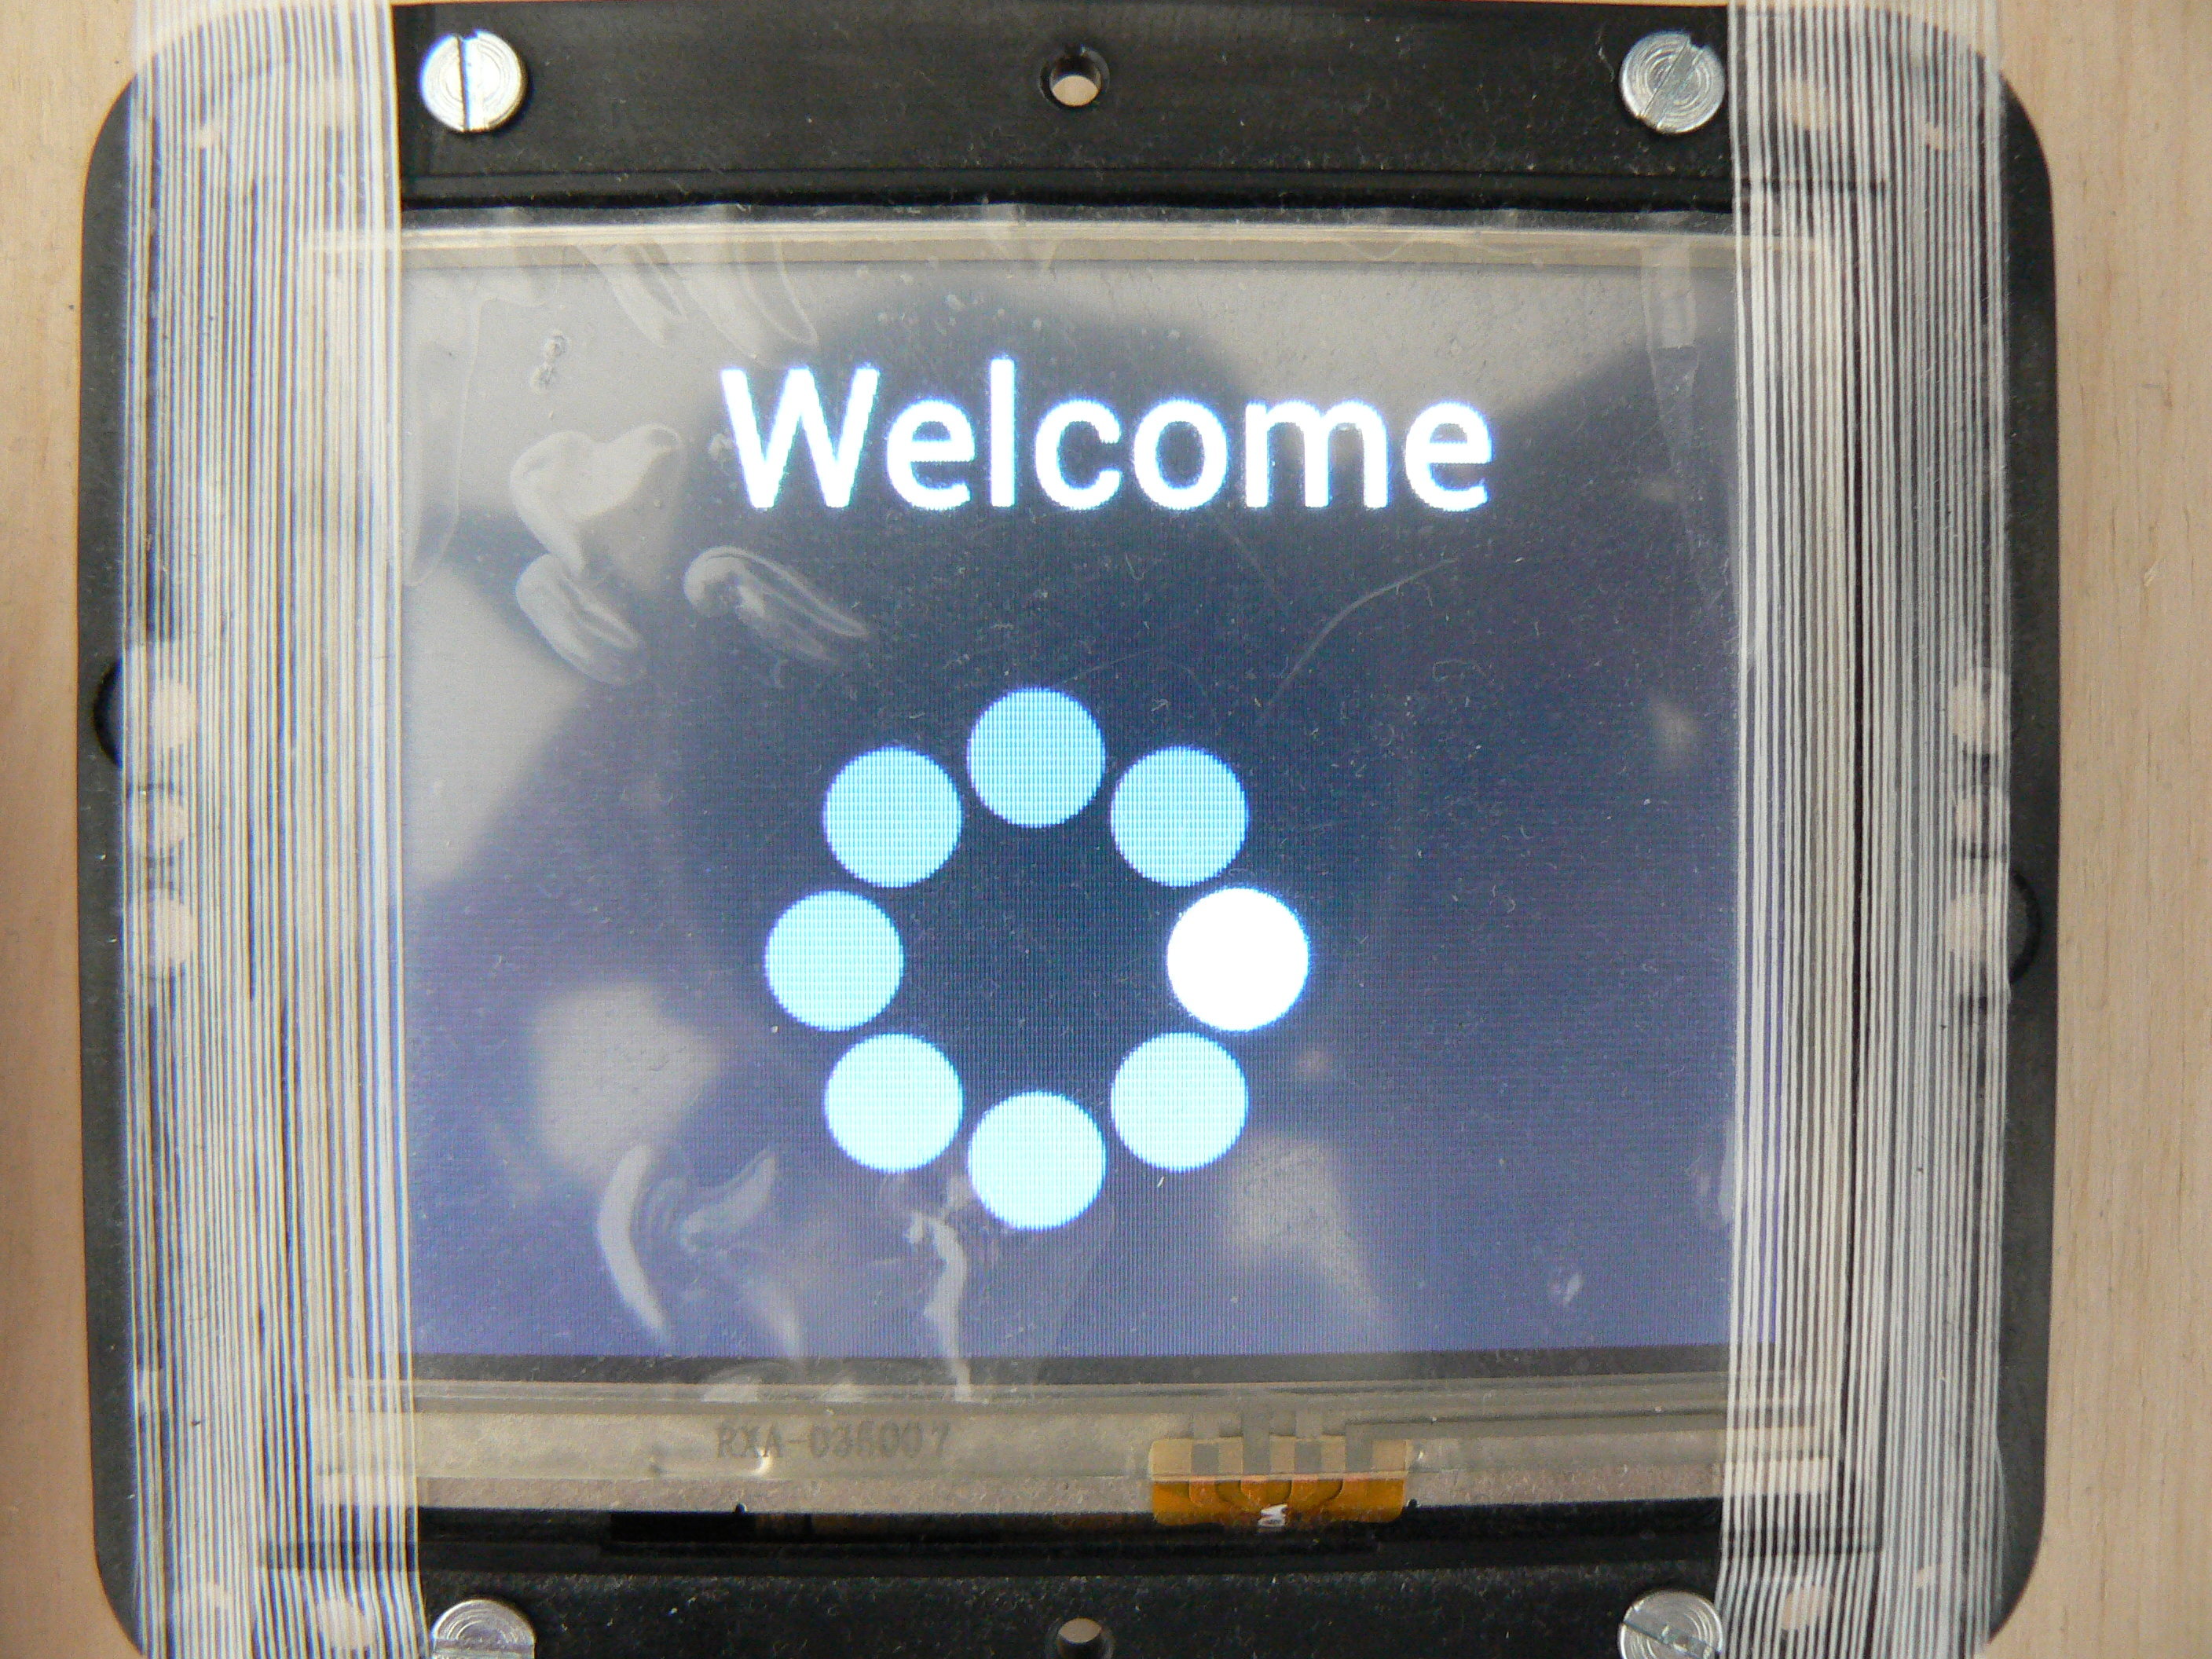
\includegraphics[height=0.3\textheight]{images/start.JPG}
    \caption{Ekran startowy}
    \source{Opracowanie własne}
\end{figure} 

Na ekranie głównym znajdują się 2 przyciski - \emph{Options} oraz \emph{Smart Mirror}. Pierwszy z nich umożliwia przejście w tryb aktywnego lusterka wstecznego, który może również służyć jako czujnik cofania co może przydać się podczas parkowania w ciasnych miejskich. Drugi pozwala na przejście do ekranu opcji systemu. 

\begin{figure}[!h]
    \centering
    	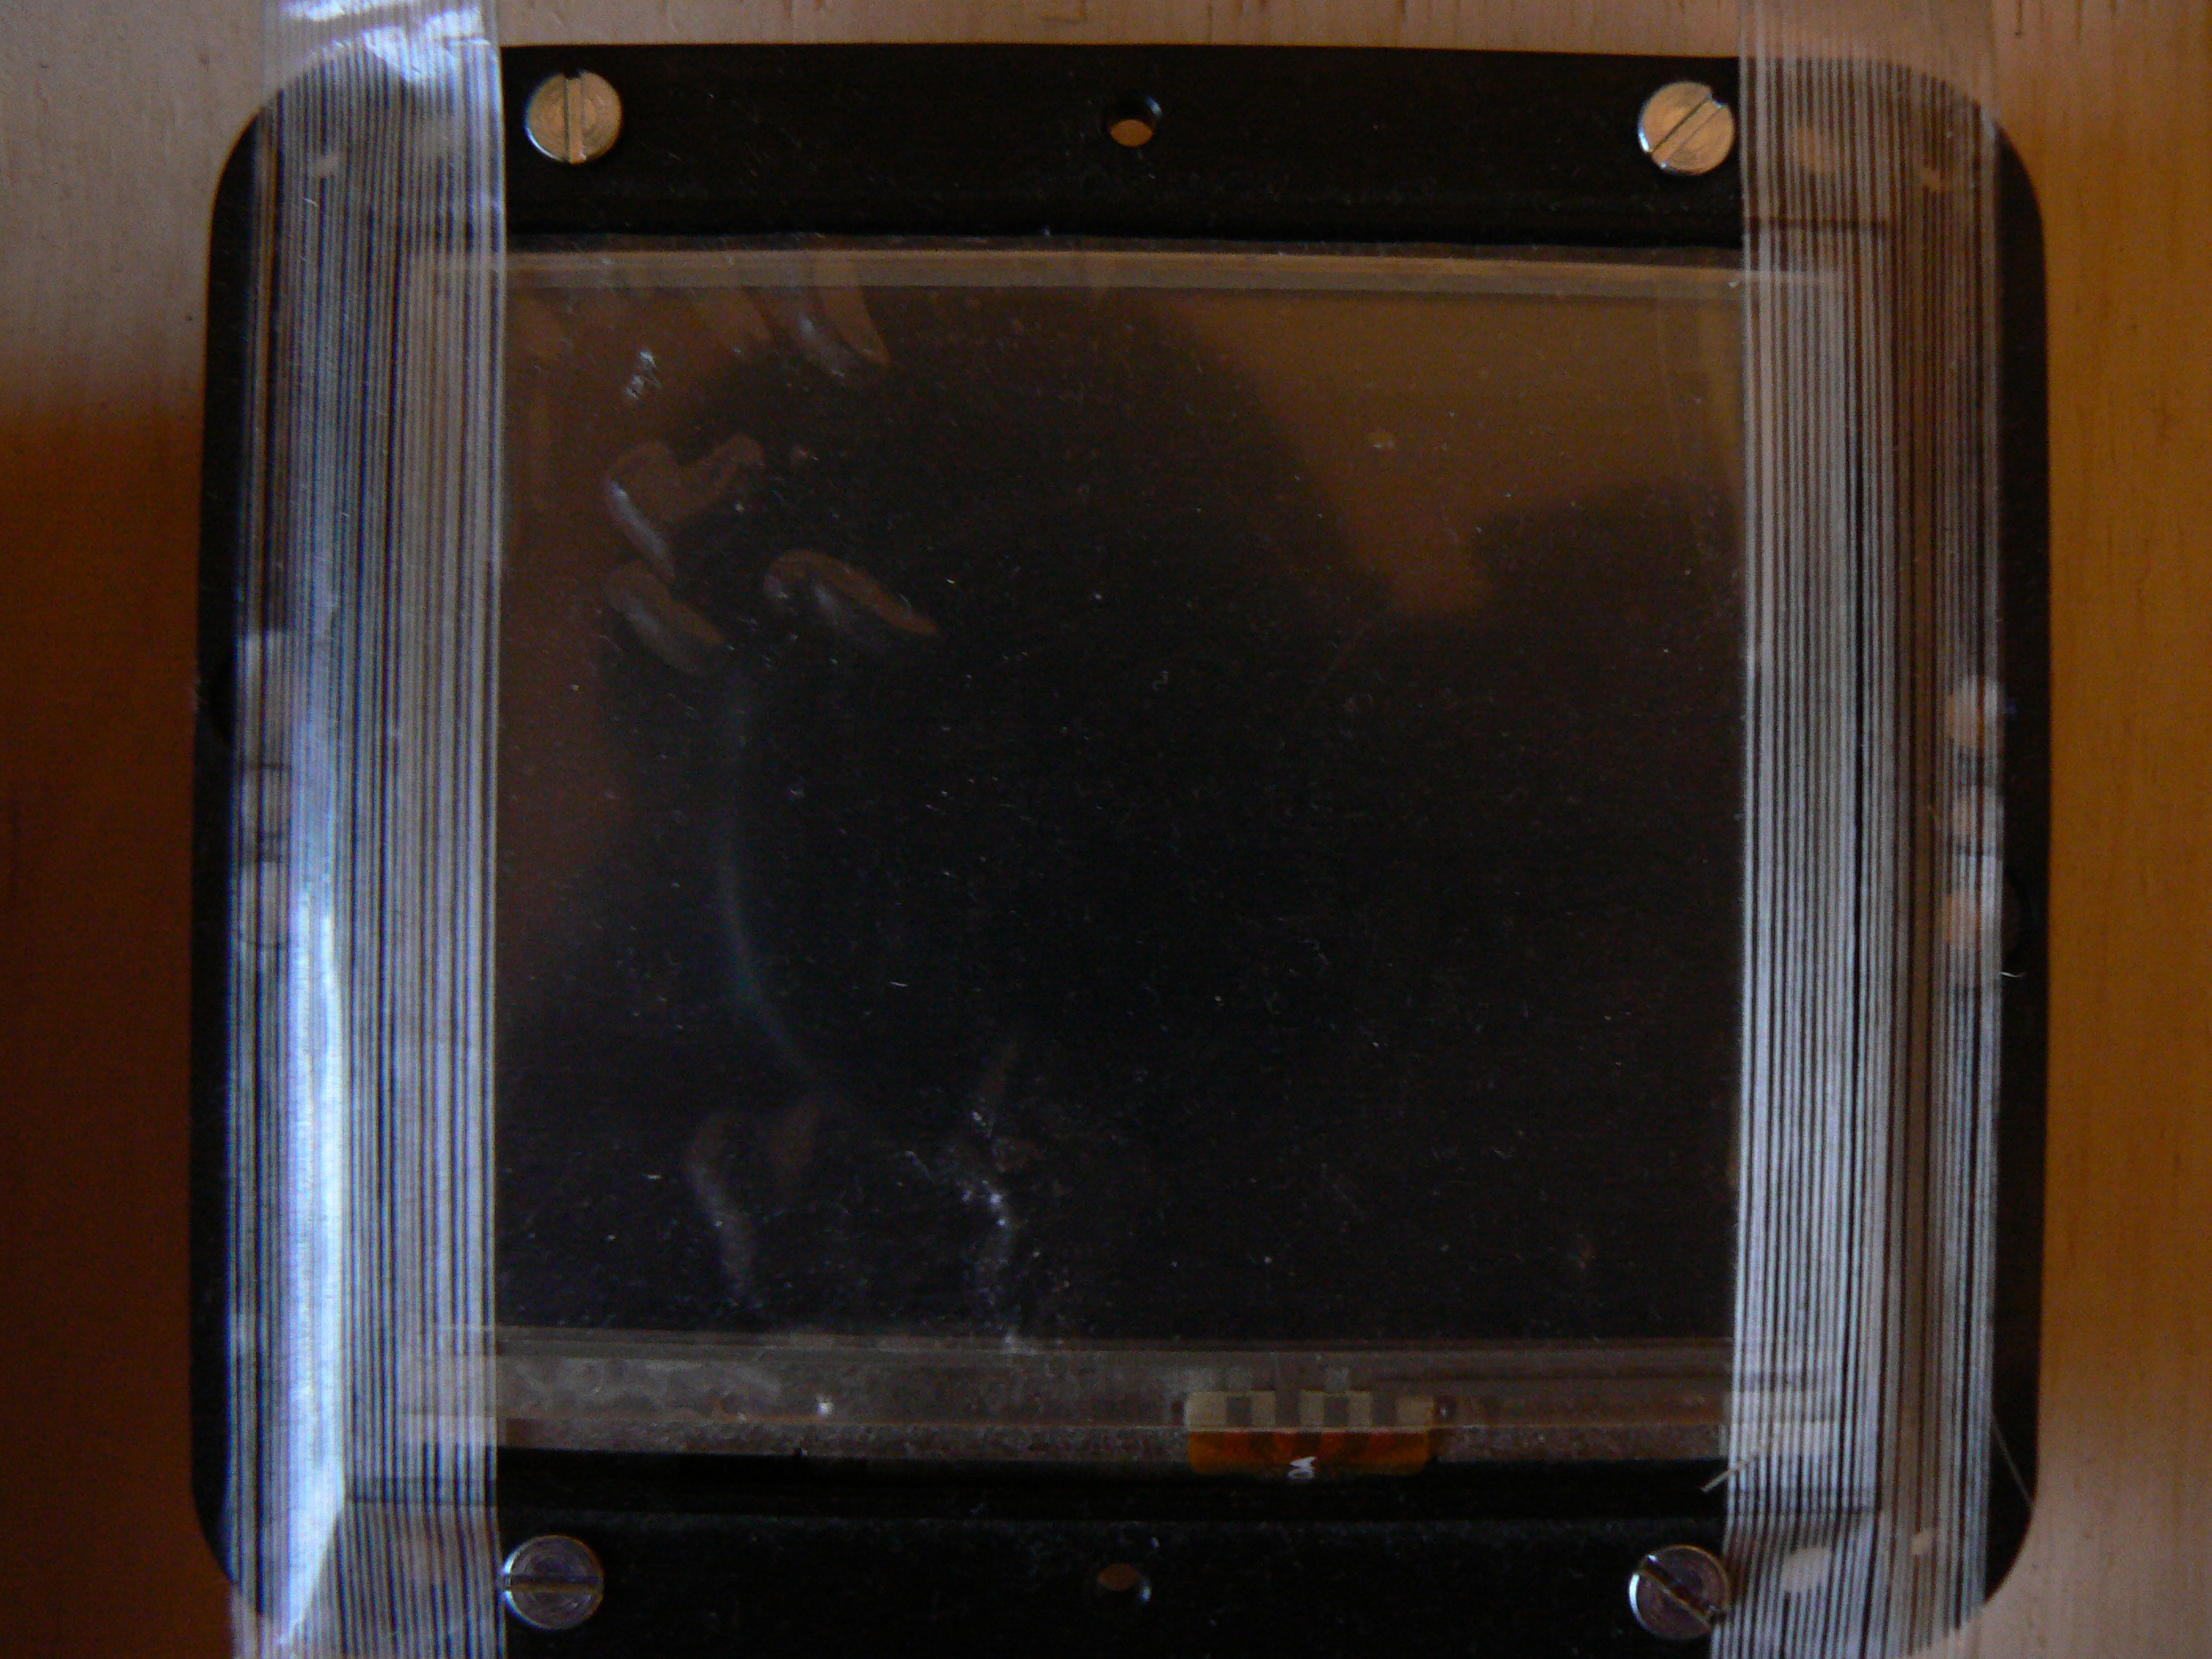
\includegraphics[height=0.3\textheight]{images/mainScreen.JPG}
    \caption{Ekran główny}
    \source{Opracowanie własne}
\end{figure}

W opcjach znajduje się możliwość rozpoczęcia zapisu danych dotyczących stanu samochodu na karcie pamięci wraz z wybranym jednym z trzech formatów zapisu danych - JSON\footnote{ang. JavaScript Object Notation - jest prostym formatem wymiany danych. Jego definicja opiera się o podzbiór języka programowania JavaScript, Standard ECMA-262 3rd Edition - December 1999. JSON jest formatem tekstowym, całkowicie niezależnym od języków programowania, ale używa konwencji, które są znane programistom korzystającym z języków z rodziny C, w tym C++, Java, JavaScript, Perl, Python i wielu innych. \cite{JSON}}, XML\footnote{ang. Extensible Markup Language. Wywodzi się od języka SGML i jest językiem znaczników służącym do opisu danych. Dane przechowywane są w postaci tekstowej w dokumencie o ściśle określonej strukturze. XML jest standardem przemysłowym i stosowany jest we wszystkich dziedzinach informatyki.\cite{XML}} oraz CSV\footnote{ang. Comma-separated values. Format przechowywania danych w postaci tekstowej. W pierwszej linii pliku znajdują się oddzielone przecinkami nazwy danych jakie są przechowywane. W kolejnych liniach wpisane są odpowiednie wartości w kolejności ustalonej przez pierwszą linie.}. Po wybraniu opcji zapisu danych, będą one zapisywane do momentu jej wyłączenia lub wyczerpania miejsca na karcie pamięci. Interwał zapisu jest również jedną z dostępnych opcji wyboru - standardowo użytkownik ma do wyboru zapis co 5s, 10s, 30s, 1 min, 15 min.

Wyłączenie systemu następuje wraz z wyłączeniem zapłonu w samochodzie. 

\begin{figure}[!h]
    \centering
    	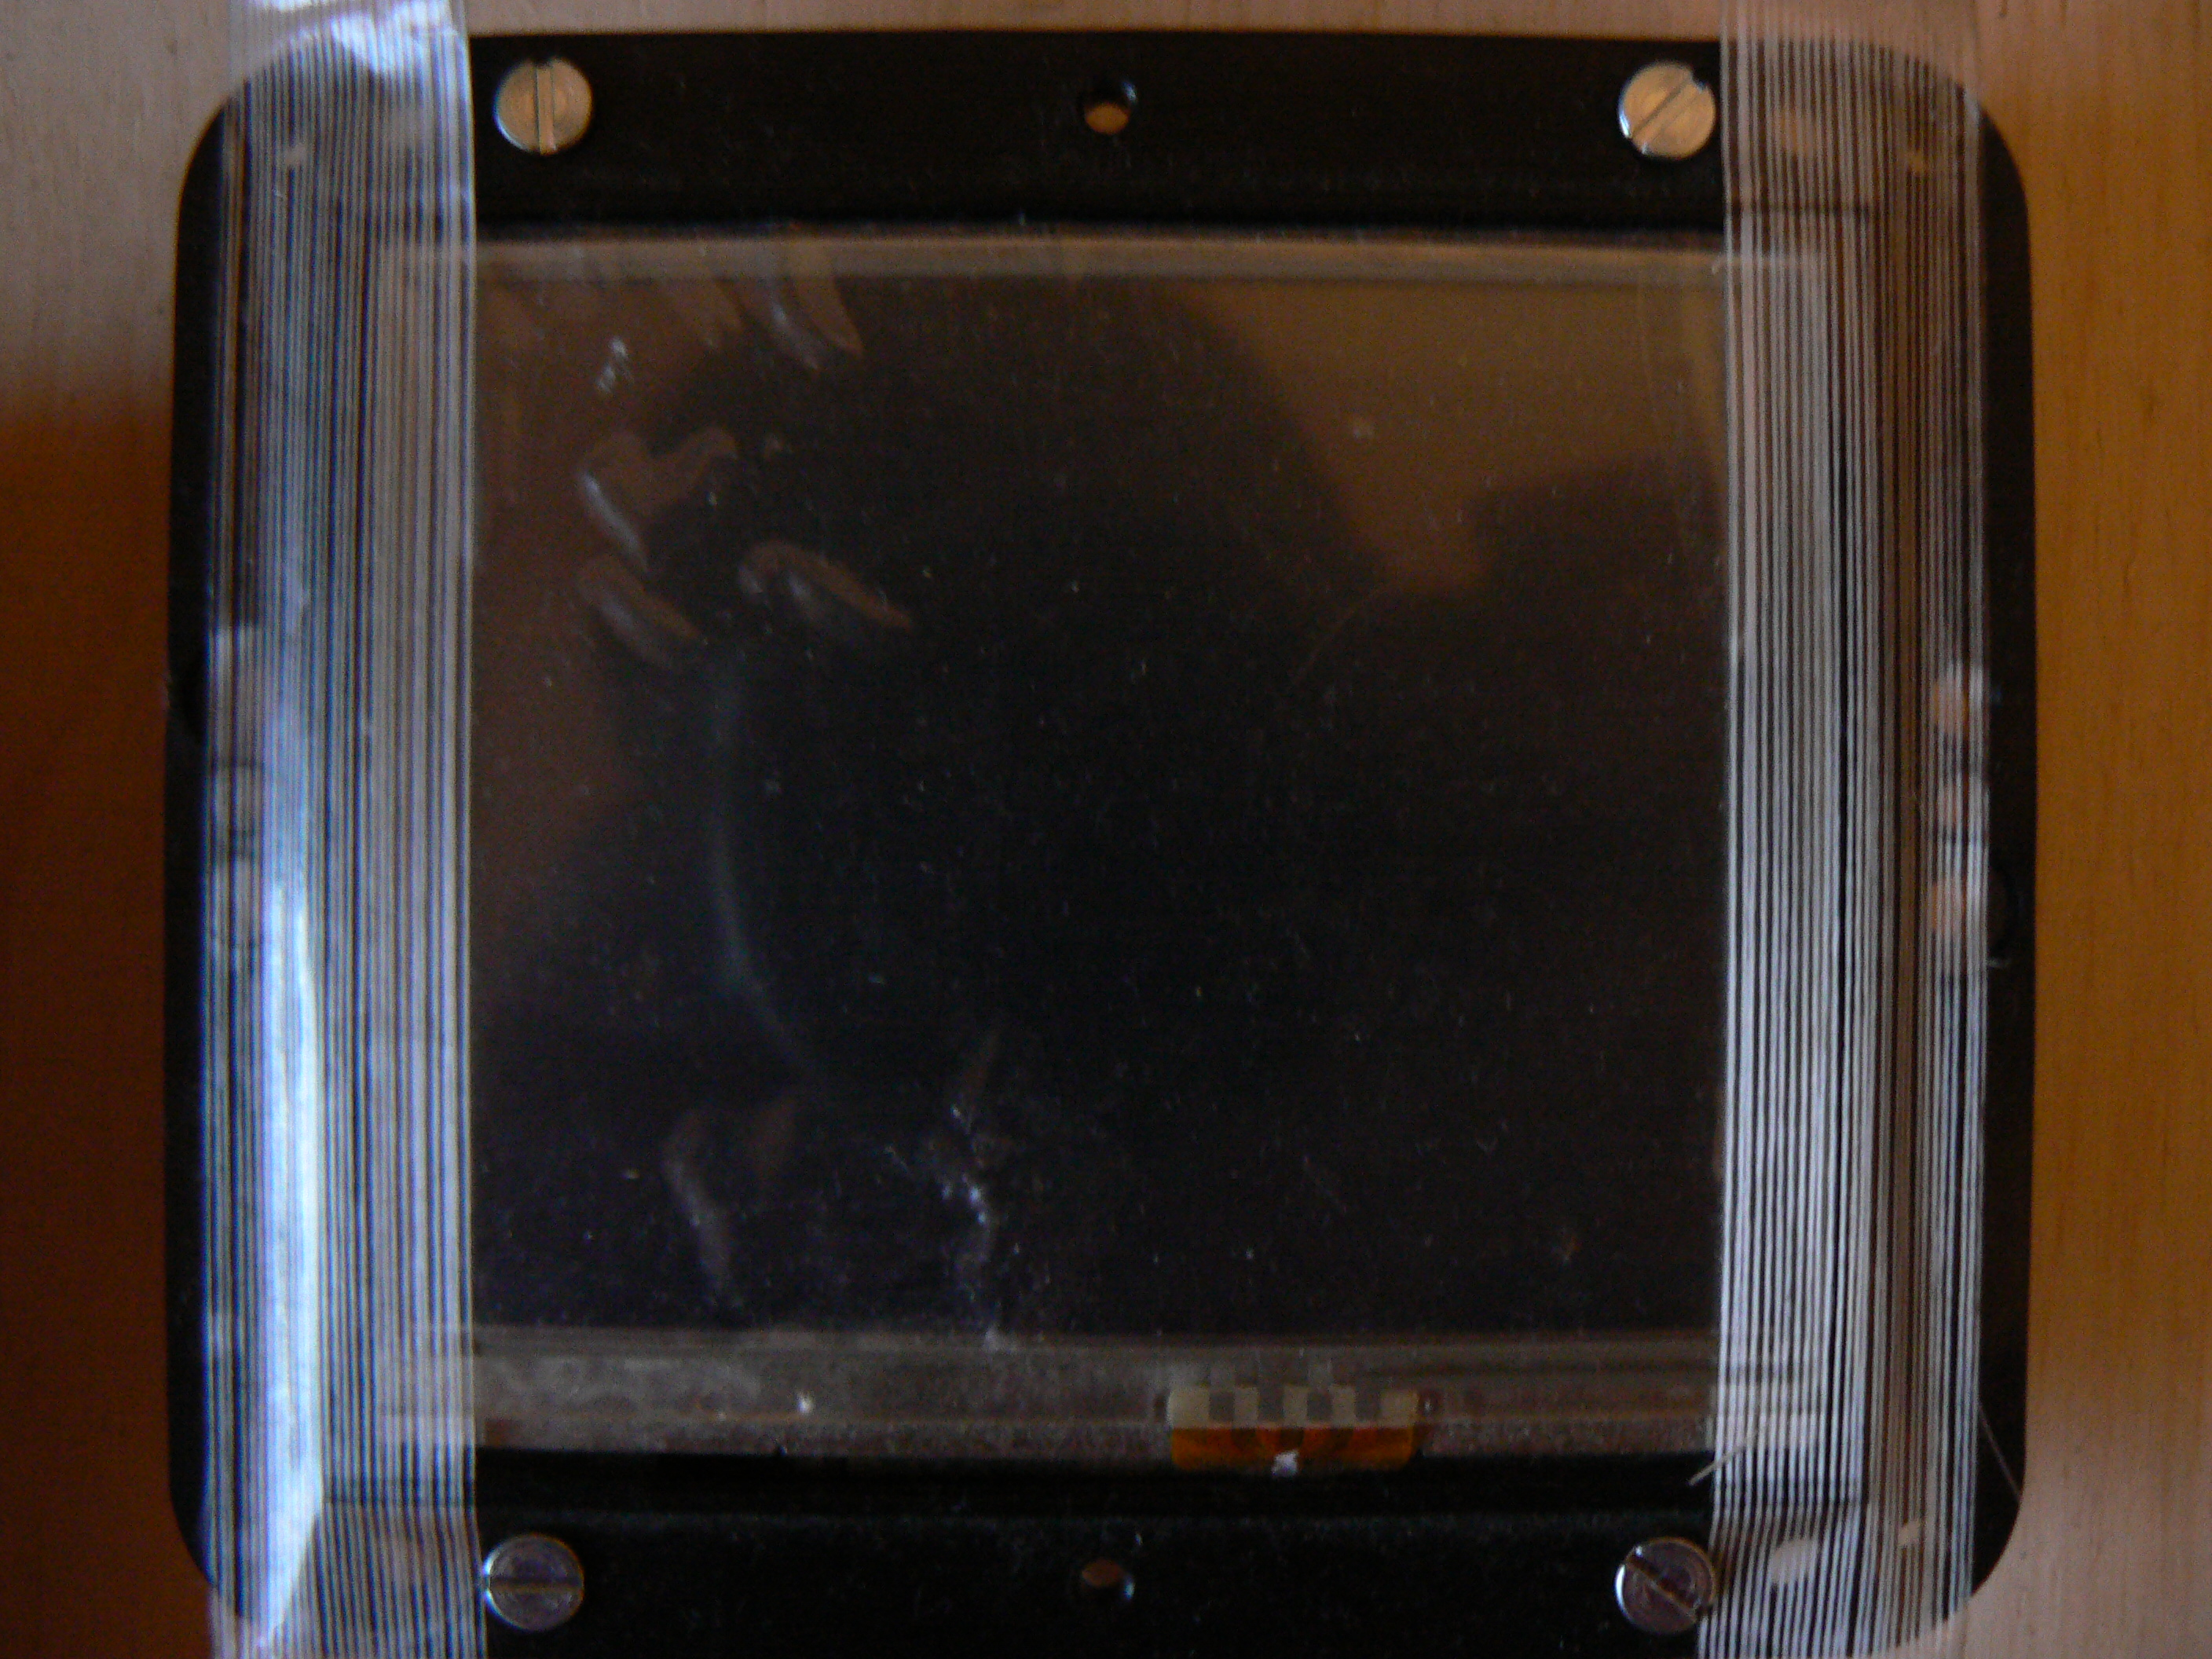
\includegraphics[height=0.3\textheight]{images/opcje.JPG}
    \caption{Ekran opcji}
    \source{Opracowanie własne}
\end{figure}

Komunikacja z Intel Galileo z ekranem odbywa się używając protokołu \emph{SPI}. Łącznie użytych zostało 7 linii: \emph{SDI}, \emph{SDO}, \emph{clock}, \emph{PD}, CS\footnote{Linia Chip Select wyświetlacza} oraz PWR\footnote{ang. Power - 5V} i \emph{GND}\footnote{ang. Ground}, natomiast komunikacja komputera z symulatorem odbywa się poprzez użycie protokołu $I^2C$. Odczytanie wartości czujników cyfrowych odbywa się po otrzymaniu przerwania sprzętowego zgłaszanego przez I/O Expander przy zmianie jakiejkolwiek wartości np. przy otworzeniu drzwi. Odczyt czujników analogowych (temperatura) odbywa się przy użyciu timera co określony w programie czas. 

Gdy została wybrana opcja zapisu danych na kartę pamięci wtedy w nieskończonej pętli w odstępach czasu wybranych przez użytkownika aktualna pozycja \emph{GPS} zostaje zapisywana do pliku tekstowego do momentu wyłączenia systemu, wyczerpania miejsca na karcie lub zmiany tej opcji przez użytkownika. Zapis do pliku odbywa się poprzez użycie standardowych funkcji języka C znajdujących się w \emph{stdlib.h}. Możliwy jest w 3 najbardziej popularnych formatach: CSV, JSON oraz XML. Format może zostać wybrany przez użytkownika poprzez zmianę w ustawieniach komputera.

\begin{lstlisting}[label=bot-dirs-alg,caption=Obsługa karty microSD za pomocą mechanizmu Arduino]
void writeSD(char *filename, char * data){
  File dataFile = SD.open(filename, FILE_WRITE);
  dataFile.println(data);
  dataFile.close();
}
void readSD(char *filename){
  File dataFile = SD.open(filename);
  while (dataFile.available()) {
      Serial.write(dataFile.read());
  }
  dataFile.close();
}
\end{lstlisting}

\begin{lstlisting}[label=bot-dirs-alg,caption=Obsługa karty microSD za pomocą mechanizmu systemu operacyjnego]
void writeSD(){
  String command = "";  
  command = "echo testTekst";
  command += " >> /tmp/daniel.txt";
  system(command.buffer);
}
\end{lstlisting}

\begin{lstlisting}[label=bot-dirs-alg,caption=Obsługa karty microSD za pomocą języka C]
  FILE *fp;
  fp = fopen("/tmp/daniel.txt", "a");
  fprintf(fp, "tekst");
  fclose(fp);
\end{lstlisting}

Intel Galileo został wyposażony w zegar czasu rzeczywistego (RTC), który został wykorzystany do zapisu danych do pliku. Dane zapisywane są do pliku, którego nazwa jest taka sama jak data. Do odczytania aktualnej daty wystarczy użyć standardowych funkcji dostępnych w języku C. Należy jednak pamiętać o tym, aby zegar był cały czas zasilany poprzez zewnętrzną baterię. W przeciwnym wypadku za każdym razem będzie on resetowany do domyślnej daty.

\begin{lstlisting}[label=bot-dirs-alg,caption=Odczyt aktualnej daty]
  system("date '+%H:%M:%S' > /tmp/time.txt");
  char buf[9];
  FILE *fp;
  fp = fopen("/tmp/time.txt", "r");
  fgets(buf, 9, fp);
  fclose(fp);
\end{lstlisting}

\begin{figure}[!hp]
    \centering
    	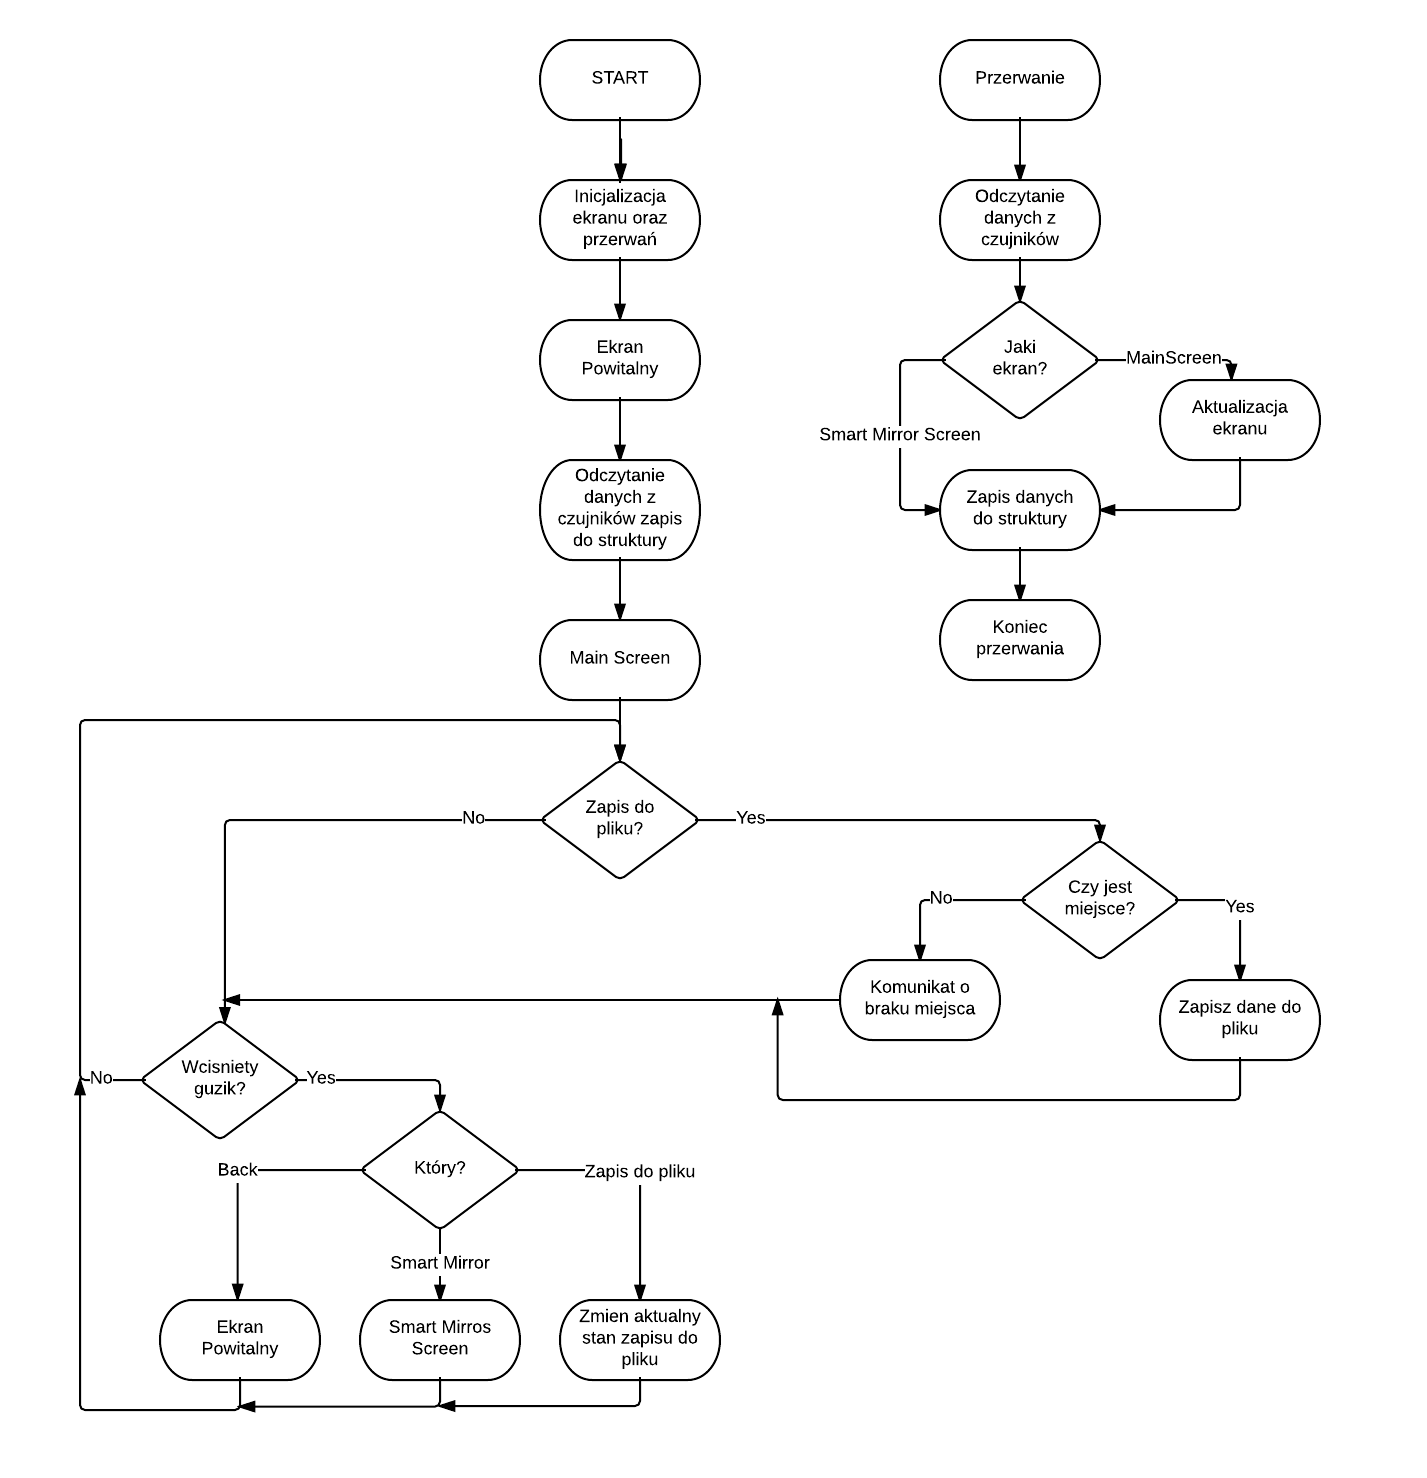
\includegraphics[height=0.6\textheight]{images/codeDiagram.png}
    \caption{Schemat blokowy działania programu}
    \source{Opracowanie własne}
\end{figure}

W systemie samochód obrazowany jest za pomocą struktury, która jako pola posiada informację na temat aktualnego stanu pojazdu. Drzwi oraz pasy zostały zobrazowane jako liczba naturalna, w której poszczególne bity oznaczają stany binarne (1 - otwarte, 0 - zamknięte).

\begin{lstlisting}[label=bot-dirs-alg,caption=Struktura samochodu w programie]
struct car {
	int doors;
 	int seatbelts;
 	int lights;         
 	int r;
 	float tempOut;
 	float tempIn;
 	float tempEngine;
};
\end{lstlisting}

\begin{table}[!tbh]
\begin{tabular}{|c|c|c|} \hline
\textbf{Port} & \textbf{Opis} & \textbf{Typ} \\ \hline
	2 & Nasłuch na przerwania z I/O Expander & Cyfrowy \\ \hline
	6 & Linia SCL & Cyfrowy \\ \hline
	7 & Linia SDA & Cyfrowy \\ \hline
	8 & Linia SDI & Cyfrowy \\ \hline
	9 & Linia SDO & Cyfrowy \\ \hline
	10 & Linia clock & Cyfrowy \\ \hline
	11 & Linia PD & Cyfrowy \\ \hline
	12 & Linia CS & Cyfrowy \\ \hline
	14 & GROUND & Cyfrowy \\ \hline
	A0 & Temperatura w środku & Analogowy \\ \hline
	A1 & Temperatura na zewnątrz & Analogowy \\ \hline
	A2 & Temperatura silnika & Analogowy \\ \hline
\end{tabular}
\caption{Porty użyte do działania systemu}
\end{table}

Dokumentacja kodu została napisana za pomocą notacji wykorzystanej w systemie \emph{DOXYGEN} i zapisana do pliku \emph{PDF}.

Dodatkowym modułem systemu jest uruchomiony na nim napisany w technologii \emph{NodeJS} serwer www udostępniający usługę śledzenia pojazdu. Gdy system zostanie podłączony do internetu (np. poprzez wejście Ethernet lub kartę Wi-Fi) użytkownik ma możliwość wejścia na stronę www gdzie może na bieżąco sprawdzać położenie samochodu na mapie oraz aktualną temperaturę wraz ze stanem drzwi oraz pasów. Komunikacja systemu z serwerem odbywa się poprzez udostępnione \emph{REST API}. Użycie technologii \emph{AngularJS} pozwala na wyświetlanie bieżących danych bez konieczności odświeżania strony.

\begin{lstlisting}[label=bot-dirs-alg,caption=Request wysyłany do serwera www]
curl -i -X POST -H 'Content-Type: application/json' -d 
'{"tempIn": "40", "tempOut" : "20", "tempEngine" : "6", 
"GPSlongitude" : "52", "GPSlatitude" : "18", 
"doors" : "5", "seatbelt" : "6", "lights" : "0" }' 
http://localhost:3000/updateData
\end{lstlisting}

Wygląd strony został przedstawiony na zrzucie ekranu poniżej.
\begin{figure}[!h]
    \centering
    	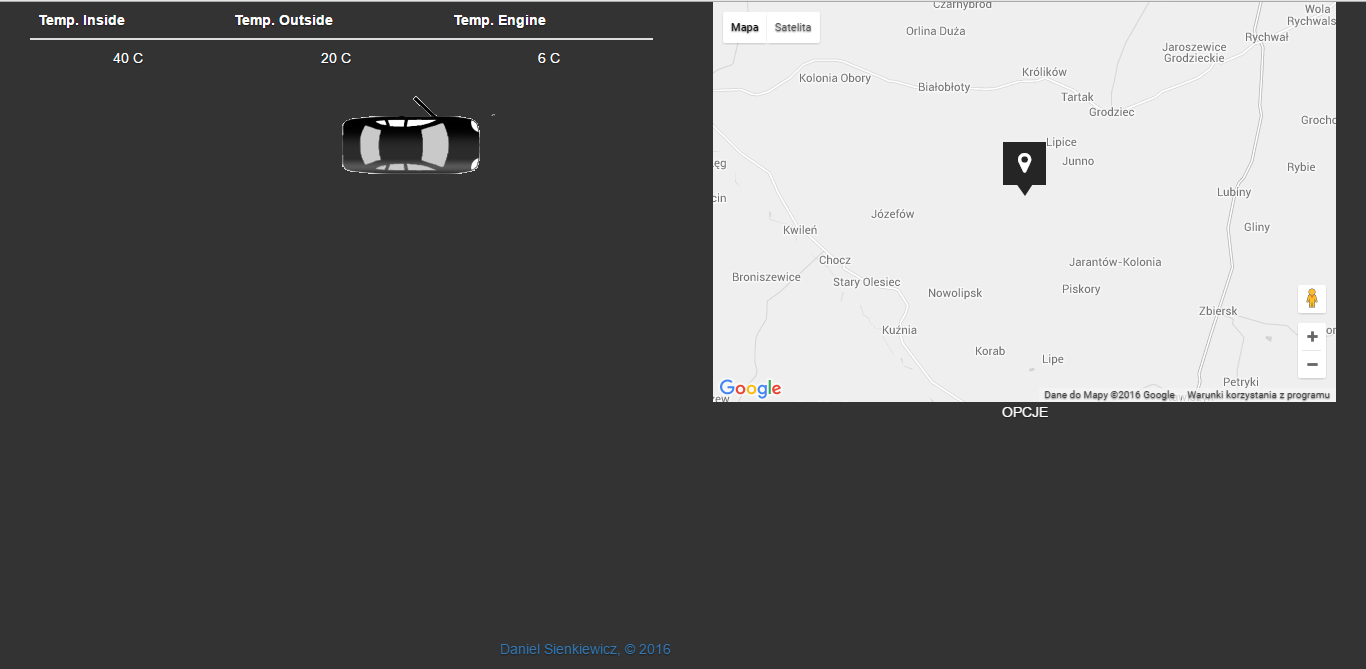
\includegraphics[height=0.35\textheight]{images/www.png}
    \caption{Strona www}
    \source{Opracowanie własne}
\end{figure}

\section{Wnioski oraz własne doświadczenia}
Komputer został tak zaprojektowany tak aby w łatwy sposób można było dodać kolejne funkcjonalności zależne od potrzeb użytkownika. Jako propozycje można uwzględnić:
\begin{enumerate}
	\item Lokalizator \emph{GPS} - wczytywanie aktualnej pozycji \emph{GPS} i wyświetlanie jej na wyświetlaczu
	\item Kamerka cofania - wyświetlanie obrazu z kamerki cofania na wyświetlaczu
	\item Czujnik deszczu - automatyczne włączenie wycieraczek i dopasowanie ich prędkości w zależności od obfitości opadów i prędkości samochodu, dodatkowe włączenie wycieraczki tylnej w momencie gdy zostanie wrzucony bieg wsteczny
	\item Sterowanie głośnością radia w zależności od prędkości samochodu
	\item Blokada immobilizer
	\item Obsługa telefonu komórkowego za pomocą bluetooth
	\item Router - dodanie modułu karty WiFi w połączeniu z odbieraniem sieci komórkowej \emph{GPRS} oraz rozsyłanie jej w samochodzie
\end{enumerate}
Jednak na potrzeby tej wersji projektu nie zostały one zaimplementowane. Oczywiście ogranicza nas tylko nasza wyobraźnia oraz finanse jakie chcemy przeznaczyć na rozbudowę systemu o dodatkowe moduły.

Intel Galileo ma wiele zalet ale niestety posiada również i wady. Największą zaletą jest możliwość obsługi systemu operacyjnego Linux oraz standard pinów \emph{GPIO} w pełni kompatybilny z popularnym Arduino co daje możliwość zakupu wielu dodatkowych dedykowanych modułów. Posiadanie pełnego systemu operacyjnego daje możliwość wykorzystania go jako na przykład serwer www lub domowego serwera multimedialnego. 

Pierwszą rzeczą na którą należy uważać jest zasilanie. Galileo ma możliwość zasilania poprzez port \emph{USB} lecz w praktyce nie jest to możliwe. Podczas uruchomienia prąd dostarczany poprzez \emph{USB} jest nie wystarczający i następuję automatyczne wyłączenie sprzętu podczas którego Software zostaje uszkodzony. Kolejną wadą jest szybkość pinów \emph{GPIO}. Są one w porównaniu do innych urządzeń dostępnych na rynku bardzo wolne co znacznie ogranicza jego możliwości.

Podczas pracy nad projektem niestety uszkodzone zostało Galileo - spalił się port USB niezbędny do ładowanie programów. Po zamianie na Galileo Gen 2 i przetestowaniu tego samego programu okazało się, że w wersji 2 znacznie poprawione zostały porty GPIO. Program, który na Gen 1 uruchamiał się w 40s, na Gen 2 uruchamia się 4s.
%================KONIEC Działanie komputera pokładowego=====================

%================Zakończenie=====================
\summary
Celem niniejszej pracy było wykonanie komputera pokładowego do samochodu bazującego na mikrokomputerze Intel Galileo oraz sprawdzenie możliwości tego mikrokomputera. Przedstawiony projekt nie jest w pełni kompletnym rozwiązaniem. Funkcjonalności takie jak określanie pozycji GPS oraz inteligentne lusterko wsteczne zostały za symulowane na potrzeby pracy.

Podczas pracy nad projektem udało się sprawdzić możliwości Intel Galileo wykorzystując rożne interfejsy komunikacyjne (porty GPIO, Ethernet, USB, RS-232) oraz możliwości systemu Linux YOCTO.

Reasumując Intel Galileo jest bardzo ciekawym rozwiązaniem w świecie IoT\footnote{ang. Internet of things - system powiązanych ze sobą urządzeń gromadzących i przetwarzających informacje najczęściej za pośrednictwem sieci komputerowej}. Posiada ogromne możliwości do wykorzystania jako na przykład domowy serwer multimedialny lub kontroler urządzeń wejścia/wyjścia. Osobiście polecałbym generację 2 ze względu na poprawioną obsługę portów GPIO co znacznie ułatwia korzystanie z nich.
%================KONIEC Zakonczenie=====================

%================Dodatki=====================
\appendix
\chapter{Karty Katalogowe}
Katalog \emph{datasheets} zawiera karty katalogowe użytych podzespołów
\begin{enumerate} 
\item Intel Galileo.pdf - Karta katalogowa Intel Galileo
\item PCF8574.pdf - Karta katalogowa I/O Expander PCF 8574N
\item VM800B.pdf - Karta katalogowa ekranu FTDI EVE VM800B
\end{enumerate}
\chapter{Porównanie dostępnych na rynku mikro kontrolerów}
\begin{table}[!tbh]
\begin{tabular}{|c|c|c|c|} \hline
 & \textbf{Intel Galileo} & \textbf{Raspberry Pi (Model B)} & \textbf{Arduino Uno} \\ \hline
Wymiary & 10cm x 7cm & 85.60mm x 56mm x 21mm & 5.59cm x 16.5cm \\ \hline
Procesor & Intel Quark X1000 & Broadcom BCM2835 & ATmega328 \\ \hline
Taktowanie & 400MHz	& 700MHz & 16 MHz\\ \hline
Cache & 16 KB & 32KB L1 cache, 128KB L2 cache & - \\ \hline
RAM & 512 SRAM & 512 SRAM & 2 kB \\ \hline
Analog I/O	& 6 & 17 & 6 \\ \hline
Digital I/O	& 14 & 8 & 14 \\ \hline
PWM	& 6 & 1 & 6 \\ \hline
\end{tabular}
\caption{Specyfikacja dostępnych na rynku mikro kontrolerów}
\source{\url{http://eu.mouser.com/applications/open-source-hardware-galileo-pi/}\cite{GalileoVSRaspberry}}
\source{\url{http://botland.com.pl/arduino-moduly-glowne/1060-arduino-uno-r3.html}\cite{Botland}}
\end{table}

\chapter{Mapowanie portów Intel Galileo na pliki w systemie Linux}
\begin{table}[!hp]
\begin{tabular}{|c|c|c|} \hline
\textbf{Quark X1000} & \textbf{Sysfs GPIO} & \textbf{Galileo/Arduino port} \\ \hline
GPORT4 BIT7 & gpio51 & IO1 \\ \hline
GPIO6 & gpio14 & IO2 \\ \hline
GPIO7 & gpio15 & IO3 \\ \hline
GPORT1 BIT4 & gpio28 & IO4 \\ \hline
GPORT0 BIT1 & gpio17 & IO5 \\ \hline
GPORT1 BIT0 & gpio24 & IO6 \\ \hline
GPORT1 BIT3 & gpio27 & IO7 \\ \hline
GPORT1 BIT2 & gpio26 & IO8 \\ \hline
GPORT0 BIT3 & gpio19 & IO9 \\ \hline
GPORT0 BIT0 & gpio16 & IO10 \\ \hline
GPORT1 BIT1 & gpio25 & IO11 \\ \hline
GPORT3 BIT2 & gpio38 & IO12 \\ \hline
GPORT3 BIT3 & gpio39 & IO13 \\ \hline
GPORT4 BIT0 & gpio44 & A0 \\ \hline
GPORT4 BIT1 & gpio45 & A1 \\ \hline
GPORT4 BIT2 & gpio46 & A2 \\ \hline
GPORT4 BIT3 & gpio47 & A3 \\ \hline
GPORT4 BIT4 & gpio48 & A4 \\ \hline
GPORT4 BIT5 & gpio49 & A5 \\ \hline
\end{tabular}
\caption{Mapowanie portów Intel Galileo na pliki w systemie Linux}
\source{\url{http://www.malinov.com/Home/sergey-s-blog}\cite{SergeySBlog}}
\end{table}

\chapter{Programy oraz dokumentacja}
Katalog \emph{Source} zawiera kod źródłowy oprogramowania stworzonego na potrzeby pracy wraz z dokumentacją 
\begin{enumerate} 
	\item VM800Galileo.ino - główny kod programu
	\item FT800.* - obsługa wyświetlacza TFT przy użyciu protokołu komunikacyjnego SPI
	\item FT800api.* - API udostępniające podstawowe funkcje systemy HMI dostępne dla wyświetlacza TFT
	\item I2C.* - obsługa I/O Expander przy użyciu protokołu komunikacyjnego $I^2C$
	\item simulator.* - komunikacja z symulatorem samochodu
	\item doc - dokumentacja kodu wygenerowana za pomocą systemu \emph{DOXYGEN} 
\end{enumerate}
%================KONIEC Dodatki=====================

\bibliographystyle{unsrt}
\bibliography{magisterka}

\listoftables

\listoffigures

\oswiadczenie

\end{document}
